%% Spice Wizard 2026 -- NeurIPS AI for Chip Design workshop submission.
%%
%% Ported from ACM/acmart format (../ACM_Journals_Primary_Article_Template/paper2026.tex)
%% to the official NeurIPS 2026 style files that ship in this directory. Content is
%% unchanged from the acmart draft; only the class, packaging, and front matter
%% follow NeurIPS conventions (single-column article, natbib citations,
%% \workshoptitle, automatic double-blind author suppression).
%%
%% Every number in the Results section is produced by bench/analyze.py over
%% bench/runs/20260809T211634Z/ and is reproducible from the released run.

% These three recent works are not present in the base bibliography shipped
% with the project. Keeping their records here makes this source self-contained
% and prevents unresolved citations in double-blind builds.
\begin{filecontents*}{provenance_refs.bib}

\end{filecontents*}

\documentclass{article}

% Numeric, compressed citations (e.g. [1,2]) to match the paper's inline
% \cite{b1,b2} usage -- must be passed before \usepackage{neurips_2026} loads
% natbib.
\PassOptionsToPackage{numbers, compress}{natbib}

% Double-blind workshop track: no [final] or [preprint] at submission time.
% This automatically suppresses \author content and prints "Anonymous
% Author(s)" instead, and adds review line numbers.
\usepackage[dblblindworkshop]{neurips_2026}
\workshoptitle{AI for Chip Design}

% The official style file hardcodes the main-conference notice for submission
% copies (only camera-ready mode surfaces \workshoptitle), which leaves a
% workshop submission footed as if it were a main-track paper. Restate the
% notice with the workshop named. The style file itself is unmodified.
\makeatletter
\renewcommand{\@noticestring}{%
  Submitted to the \@neuripsordinal\/ Conference on Neural Information
  Processing Systems (NeurIPS \@neuripsyear) Workshop: \@workshoptitle.
  Do not distribute.%
}
\makeatother

\usepackage[utf8]{inputenc}
\usepackage[T1]{fontenc}
\usepackage{textcomp}
% hidelinks: the default draws coloured boxes around every link, which print
% badly and clutter the review copy.
\usepackage[hidelinks]{hyperref}
\usepackage{url}
\usepackage{booktabs}
\usepackage{amsfonts}
\usepackage{amsmath}
\usepackage{nicefrac}
\usepackage{microtype}
\usepackage{xcolor}
\usepackage{graphicx}
\graphicspath{{figures/}}
\usepackage{tikz}
\usetikzlibrary{arrows.meta,positioning,fit,backgrounds}
\usepackage{array}
\usepackage{multirow}
\usepackage{listings}
\usepackage[htt]{hyphenat}
\usepackage{xurl}
\def\UrlFont{\ttfamily}
\usepackage{enumitem}
\setlist[itemize]{leftmargin=*, itemsep=2pt, topsep=2pt}
\emergencystretch=2em

\lstdefinelanguage{Spice}{
  morekeywords={.subckt, .ends, .lib, .inc, .model},
  morecomment=[l]{*},
  morestring=[b]",
}
% xleftmargin keeps the listing frame clear of the submission line numbers,
% which otherwise collide with the frame rule in the left margin.
\lstset{
  language=Spice, basicstyle=\scriptsize\ttfamily,
  keywordstyle=\color{blue}\bfseries, commentstyle=\color{gray}\itshape,
  frame=single, breaklines=true, captionpos=b,
  xleftmargin=1.5em, framexleftmargin=1.5em, aboveskip=6pt, belowskip=4pt,
}

%% ===========================================================================
%% GENERATED VALUES -- pasted inline so this file compiles standalone (e.g. on
%% Overleaf) with no external dependency. DO NOT hand-edit a number here.
%% Regenerate with:
%%     python bench/reconcile.py 20260809T211634Z --out Neurips/generated
%%     python bench/mutants.py --parts 40
%% then replace the blocks below with generated/{numbers,factorial,extra,
%% mutants}.tex. reconcile.py refuses to emit if the corpus fails an integrity
%% check, so a number here disagreeing with the corpus is a build failure
%% rather than a silent discrepancy.
%% ===========================================================================
%% ==== from generated/numbers.tex ====
\newcommand{\NumAttempted}{360}
\newcommand{\NumExcluded}{18}
\newcommand{\NumNoCompletion}{26}
\newcommand{\NumNetlists}{316}
\newcommand{\NumNotConverged}{187}
\newcommand{\NumConverged}{129}
\newcommand{\NumNumericFail}{29}
\newcommand{\NumNumericPass}{100}
\newcommand{\GuardRejects}{316}
\newcommand{\GuardRejectsPasses}{100}
\newcommand{\FlagSubstituted}{98}
\newcommand{\FlagStub}{78}
\newcommand{\FlagNoPart}{15}
\newcommand{\FlagPinRole}{53}
\newcommand{\PinCountMismatch}{59}
\newcommand{\PinRolePassing}{12}
\newcommand{\PinRoleBarePassing}{11}
\newcommand{\PinRoleLibPassing}{1}
\newcommand{\BareAttempted}{171}
\newcommand{\BareNetlists}{168}
\newcommand{\BarePasses}{73}
\newcommand{\BareFalse}{71}
\newcommand{\BareFalseRate}{97}
\newcommand{\BareGenuine}{19}
\newcommand{\BareGenuineRate}{11}
\newcommand{\LibAttempted}{171}
\newcommand{\LibNetlists}{148}
\newcommand{\LibNoCompletion}{23}
\newcommand{\LibPasses}{27}
\newcommand{\LibFalse}{8}
\newcommand{\LibFalseRate}{30}
\newcommand{\LibGenuine}{146}
\newcommand{\LibGenuineRate}{99}
\newcommand{\AuditFlagged}{71}
\newcommand{\AuditCleared}{29}
\newcommand{\ClearedGraded}{29}
\newcommand{\ClearedGradedFake}{9}
\newcommand{\ClearedGradedReal}{20}
\newcommand{\ClearedMeasured}{0}
\newcommand{\ClearedUnresolved}{0}
\newcommand{\FalseAcceptTotal}{79}
\newcommand{\FalseAcceptRate}{79}
\newcommand{\ConfTP}{70}
\newcommand{\ConfFP}{1}
\newcommand{\ConfFN}{9}
\newcommand{\ConfTN}{20}
\newcommand{\AuditPrecision}{99}
\newcommand{\AuditRecall}{89}
\newcommand{\AuditSpecificity}{95}
\newcommand{\AuditFOne}{93}
\newcommand{\AuditAccuracy}{90}
\newcommand{\WaveEvaluated}{15}
\newcommand{\LabelledReal}{21}
\newcommand{\FalseAcceptCILo}{65}
\newcommand{\FalseAcceptCIHi}{92}
\newcommand{\BareFalseCILo}{91}
\newcommand{\BareFalseCIHi}{100}
\newcommand{\LibFalseCILo}{12}
\newcommand{\LibFalseCIHi}{48}
\newcommand{\BareValidPass}{2}
\newcommand{\LibValidPass}{19}
\newcommand{\BareValidRate}{1.2}
\newcommand{\LibValidRate}{11.1}
\newcommand{\BareGenuineRateAtt}{11}
\newcommand{\LibGenuineRateAtt}{85}

%% ==== from generated/factorial.tex ====
\newcommand{\FactBareAtt}{171}
\newcommand{\FactBareNoComp}{3}
\newcommand{\FactBareNet}{168}
\newcommand{\FactBareConv}{83}
\newcommand{\FactBarePass}{73}
\newcommand{\FactBareFalse}{70}
\newcommand{\FactBareRef}{19}
\newcommand{\FactBareRes}{4}
\newcommand{\FactBareRefRate}{11}
\newcommand{\FactBareResRate}{2}
\newcommand{\FactBareResRateItt}{2}
\newcommand{\FactBareResCILo}{0}
\newcommand{\FactBareResCIHi}{5}
\newcommand{\FactBareRefCILo}{4}
\newcommand{\FactBareRefCIHi}{19}
\newcommand{\FactRequirementAtt}{171}
\newcommand{\FactRequirementNoComp}{5}
\newcommand{\FactRequirementNet}{166}
\newcommand{\FactRequirementConv}{10}
\newcommand{\FactRequirementPass}{6}
\newcommand{\FactRequirementFalse}{0}
\newcommand{\FactRequirementRef}{124}
\newcommand{\FactRequirementRes}{32}
\newcommand{\FactRequirementRefRate}{75}
\newcommand{\FactRequirementResRate}{19}
\newcommand{\FactRequirementResRateItt}{19}
\newcommand{\FactRequirementResCILo}{8}
\newcommand{\FactRequirementResCIHi}{32}
\newcommand{\FactRequirementRefCILo}{70}
\newcommand{\FactRequirementRefCIHi}{79}
\newcommand{\FactLibraryAtt}{171}
\newcommand{\FactLibraryNoComp}{23}
\newcommand{\FactLibraryNet}{148}
\newcommand{\FactLibraryConv}{46}
\newcommand{\FactLibraryPass}{27}
\newcommand{\FactLibraryFalse}{1}
\newcommand{\FactLibraryRef}{146}
\newcommand{\FactLibraryRes}{141}
\newcommand{\FactLibraryRefRate}{99}
\newcommand{\FactLibraryResRate}{95}
\newcommand{\FactLibraryResRateItt}{82}
\newcommand{\FactLibraryResCILo}{90}
\newcommand{\FactLibraryResCIHi}{99}
\newcommand{\FactLibraryRefCILo}{97}
\newcommand{\FactLibraryRefCIHi}{100}
\newcommand{\FactBareClaudeAtt}{57}
\newcommand{\FactBareClaudeNoComp}{3}
\newcommand{\FactBareClaudeNet}{54}
\newcommand{\FactBareClaudeRef}{3}
\newcommand{\FactBareClaudeRefRate}{6}
\newcommand{\FactRequirementClaudeAtt}{57}
\newcommand{\FactRequirementClaudeNoComp}{0}
\newcommand{\FactRequirementClaudeNet}{57}
\newcommand{\FactRequirementClaudeRef}{56}
\newcommand{\FactRequirementClaudeRefRate}{98}
\newcommand{\FactLibraryClaudeAtt}{57}
\newcommand{\FactLibraryClaudeNoComp}{20}
\newcommand{\FactLibraryClaudeNet}{37}
\newcommand{\FactLibraryClaudeRef}{37}
\newcommand{\FactLibraryClaudeRefRate}{100}
\newcommand{\FactBareGeminiAtt}{57}
\newcommand{\FactBareGeminiNoComp}{0}
\newcommand{\FactBareGeminiNet}{57}
\newcommand{\FactBareGeminiRef}{12}
\newcommand{\FactBareGeminiRefRate}{21}
\newcommand{\FactRequirementGeminiAtt}{57}
\newcommand{\FactRequirementGeminiNoComp}{4}
\newcommand{\FactRequirementGeminiNet}{53}
\newcommand{\FactRequirementGeminiRef}{12}
\newcommand{\FactRequirementGeminiRefRate}{23}
\newcommand{\FactLibraryGeminiAtt}{57}
\newcommand{\FactLibraryGeminiNoComp}{0}
\newcommand{\FactLibraryGeminiNet}{57}
\newcommand{\FactLibraryGeminiRef}{57}
\newcommand{\FactLibraryGeminiRefRate}{100}
\newcommand{\FactBareGptAtt}{57}
\newcommand{\FactBareGptNoComp}{0}
\newcommand{\FactBareGptNet}{57}
\newcommand{\FactBareGptRef}{4}
\newcommand{\FactBareGptRefRate}{7}
\newcommand{\FactRequirementGptAtt}{57}
\newcommand{\FactRequirementGptNoComp}{1}
\newcommand{\FactRequirementGptNet}{56}
\newcommand{\FactRequirementGptRef}{56}
\newcommand{\FactRequirementGptRefRate}{100}
\newcommand{\FactLibraryGptAtt}{57}
\newcommand{\FactLibraryGptNoComp}{3}
\newcommand{\FactLibraryGptNet}{54}
\newcommand{\FactLibraryGptRef}{52}
\newcommand{\FactLibraryGptRefRate}{96}

%% ==== from generated/extra.tex ====
\newcommand{\CorpusTotal}{540}
\newcommand{\CorpusExcluded}{27}
\newcommand{\CorpusScored}{513}
\newcommand{\CorpusArms}{3}
\newcommand{\ArmAttempted}{180}
\newcommand{\ArmScored}{171}
\newcommand{\NumCases}{20}
\newcommand{\NumModels}{3}
\newcommand{\SamplesPerCell}{3}
\newcommand{\ProvTP}{70}
\newcommand{\ProvFP}{0}
\newcommand{\ProvFN}{9}
\newcommand{\ProvTN}{21}
\newcommand{\ProvPrecision}{100}
\newcommand{\ProvRecall}{89}
\newcommand{\MinimalSubsetSize}{1}
\newcommand{\MinimalSubsetFP}{0}
\newcommand{\GroundsFakeSubckt}{62}
\newcommand{\GroundsFakeNoInstance}{8}
\newcommand{\GroundsFakeRead}{9}
\newcommand{\GroundsValidDistortion}{10}
\newcommand{\GroundsValidRead}{11}
\newcommand{\StageProvAccepted}{30}
\newcommand{\StageIfaceAccepted}{29}
\newcommand{\StageWaveAccepted}{29}
\newcommand{\StageWaveRemoved}{0}
\newcommand{\WaveViolations}{1}
\newcommand{\StageNumericFalseShare}{79}
\newcommand{\StageNumericValidShare}{21}
\newcommand{\StageProvFalseShare}{30}
\newcommand{\StageProvValidShare}{70}
\newcommand{\StageIfaceFalseShare}{31}
\newcommand{\StageIfaceValidShare}{69}
\newcommand{\StageWaveFalseShare}{31}
\newcommand{\StageWaveValidShare}{69}
\newcommand{\SoloNoPartFlagged}{8}
\newcommand{\SoloNoPartPrecision}{100}
\newcommand{\SoloNoPartTP}{8}
\newcommand{\SoloNoPartFP}{0}
\newcommand{\SoloNoPartRecall}{10}
\newcommand{\UniqueNoPart}{0}
\newcommand{\SoloSubstitutedFlagged}{62}
\newcommand{\SoloSubstitutedPrecision}{100}
\newcommand{\SoloSubstitutedTP}{62}
\newcommand{\SoloSubstitutedFP}{0}
\newcommand{\SoloSubstitutedRecall}{78}
\newcommand{\UniqueSubstituted}{0}
\newcommand{\SoloBehavioralStubFlagged}{46}
\newcommand{\SoloBehavioralStubPrecision}{100}
\newcommand{\SoloBehavioralStubTP}{46}
\newcommand{\SoloBehavioralStubFP}{0}
\newcommand{\SoloBehavioralStubRecall}{58}
\newcommand{\UniqueBehavioralStub}{0}
\newcommand{\SoloResolvedBindingFlagged}{70}
\newcommand{\SoloResolvedBindingPrecision}{100}
\newcommand{\SoloResolvedBindingTP}{70}
\newcommand{\SoloResolvedBindingFP}{0}
\newcommand{\SoloResolvedBindingRecall}{89}
\newcommand{\UniqueResolvedBinding}{0}
\newcommand{\SoloPinRoleMismatchFlagged}{12}
\newcommand{\SoloPinRoleMismatchPrecision}{92}
\newcommand{\SoloPinRoleMismatchTP}{11}
\newcommand{\SoloPinRoleMismatchFP}{1}
\newcommand{\SoloPinRoleMismatchRecall}{14}
\newcommand{\UniquePinRoleMismatch}{0}
\newcommand{\PassOneBareNumeric}{42.7}
\newcommand{\PassKBareNumeric}{56.1}
\newcommand{\PassOneBareNumericCI}{[32.2,52.6]}
\newcommand{\PassKBareNumericCI}{[43.9,68.4]}
\newcommand{\PassOneBareProv}{1.8}
\newcommand{\PassKBareProv}{3.5}
\newcommand{\PassOneBareProvCI}{[0.0,4.7]}
\newcommand{\PassKBareProvCI}{[0.0,8.8]}
\newcommand{\PassOneBareFull}{1.8}
\newcommand{\PassKBareFull}{3.5}
\newcommand{\PassOneBareFullCI}{[0.0,4.7]}
\newcommand{\PassKBareFullCI}{[0.0,8.8]}
\newcommand{\PairedDropBareOne}{[31.0,50.9]}
\newcommand{\PairedDropBareK}{[40.4,63.2]}
\newcommand{\PassOneLibNumeric}{15.8}
\newcommand{\PassKLibNumeric}{22.8}
\newcommand{\PassOneLibNumericCI}{[6.4,26.9]}
\newcommand{\PassKLibNumericCI}{[10.5,36.8]}
\newcommand{\PassOneLibProv}{15.8}
\newcommand{\PassKLibProv}{22.8}
\newcommand{\PassOneLibProvCI}{[6.4,26.9]}
\newcommand{\PassKLibProvCI}{[10.5,36.8]}
\newcommand{\PassOneLibFull}{15.2}
\newcommand{\PassKLibFull}{22.8}
\newcommand{\PassOneLibFullCI}{[5.8,25.7]}
\newcommand{\PassKLibFullCI}{[10.5,36.8]}
\newcommand{\PairedDropLibOne}{[0.0,0.0]}
\newcommand{\PairedDropLibK}{[0.0,0.0]}
\newcommand{\PassOneReqNumeric}{3.5}
\newcommand{\PassKReqNumeric}{5.3}
\newcommand{\PassOneReqNumericCI}{[0.0,9.9]}
\newcommand{\PassKReqNumericCI}{[0.0,14.0]}
\newcommand{\PassOneReqProv}{3.5}
\newcommand{\PassKReqProv}{5.3}
\newcommand{\PassOneReqProvCI}{[0.0,9.9]}
\newcommand{\PassKReqProvCI}{[0.0,14.0]}
\newcommand{\PassOneReqFull}{3.5}
\newcommand{\PassKReqFull}{5.3}
\newcommand{\PassOneReqFullCI}{[0.0,9.9]}
\newcommand{\PassKReqFullCI}{[0.0,14.0]}
\newcommand{\PairedDropReqOne}{[0.0,0.0]}
\newcommand{\PairedDropReqK}{[0.0,0.0]}

%% ==== from generated/mutants.tex ====
\newcommand{\MutParts}{40}
\newcommand{\MutTotal}{360}
\newcommand{\MutClasses}{9}
\newcommand{\MutTP}{262}
\newcommand{\MutFP}{0}
\newcommand{\MutFN}{18}
\newcommand{\MutTN}{80}
\newcommand{\MutPrecision}{100}
\newcommand{\MutRecall}{94}
\newcommand{\MutProvPrecision}{100}
\newcommand{\MutProvRecall}{86}
\newcommand{\MutIdentityN}{40}
\newcommand{\MutIdentityFlagged}{0}
\newcommand{\MutIdentityRate}{0}
\newcommand{\MutWrapperN}{40}
\newcommand{\MutWrapperFlagged}{0}
\newcommand{\MutWrapperRate}{0}
\newcommand{\MutSubstituteN}{40}
\newcommand{\MutSubstituteFlagged}{40}
\newcommand{\MutSubstituteRate}{100}
\newcommand{\MutRenamedStubN}{40}
\newcommand{\MutRenamedStubFlagged}{40}
\newcommand{\MutRenamedStubRate}{100}
\newcommand{\MutShadowN}{40}
\newcommand{\MutShadowFlagged}{40}
\newcommand{\MutShadowRate}{100}
\newcommand{\MutDropLibraryN}{40}
\newcommand{\MutDropLibraryFlagged}{40}
\newcommand{\MutDropLibraryRate}{100}
\newcommand{\MutRemovePartN}{40}
\newcommand{\MutRemovePartFlagged}{40}
\newcommand{\MutRemovePartRate}{100}
\newcommand{\MutAliasFileN}{40}
\newcommand{\MutAliasFileFlagged}{40}
\newcommand{\MutAliasFileRate}{100}
\newcommand{\MutPinPermuteN}{40}
\newcommand{\MutPinPermuteFlagged}{22}
\newcommand{\MutPinPermuteRate}{55}

%% ===========================================================================
%% ARTIFACT URL -- the ONE place to edit. Submission is double-blind, so this
%% must be an anonymised mirror (e.g. anonymous.4open.science), never a
%% personal GitHub URL, which de-anonymises the authors. Swap to the canonical
%% repository URL for camera-ready.
%% ===========================================================================
\newcommand{\artifacturl}{\texttt{<ANONYMISED ARTIFACT URL: REPLACE BEFORE SUBMITTING>}}

\title{Simulation-Verified Is Not Provenance-Verified: Provenance-Qualified
  Evaluation for LLM Analog Netlist Generation}

%% Double-blind: the dblblindworkshop track option prints "Anonymous
%% Author(s)" regardless of this block's contents, so the placeholder below
%% never appears in the compiled PDF. Kept non-empty because \author{} must
%% not be blank.
\author{%
  Anonymous Author(s) \\
  Anonymous Institution \\
  \texttt{anonymous@example.org}
}

\begin{document}

\maketitle
\begin{abstract}
Simulator-in-the-loop generation is the prevailing paradigm for LLM-based
analog netlist generation: a model proposes a netlist, a SPICE simulation
measures it, and the netlist is accepted if it meets its numeric target. We
examine what this acceptance criterion actually certifies. Across
\NumNetlists{} netlists generated by three frontier models on a 20-part
stress-test suite of vendor ICs, \BareFalse{} of \BarePasses{} unprompted
numeric passes (\BareFalseRate{}\%, 95\% confidence interval (CI)
\BareFalseCILo{}--\BareFalseCIHi{}\%) are false acceptances: the
manufacturer's model of the requested part did not produce the measured
result. In the commonest case the part is replaced by a locally defined
behavioural subcircuit reproducing the target value but none of the
characteristics the part is specified for; manual grading of all
\NumNumericPass{} numeric passes yields
\FalseAcceptTotal{}/\NumNumericPass{} false acceptances (\FalseAcceptRate{}\%,
95\% CI \FalseAcceptCILo{}--\FalseAcceptCIHi{}\%). Read as Pass@$k$ over
identical generations, requiring the part name to resolve to a
vendor-supplied definition moves unprompted Pass@1 from
\PassOneBareNumeric{}\% to \PassOneBareProv{}\%. Two prompt ablations separate
an explicit no-substitution \emph{requirement} from \emph{availability} of the
loading directive: prohibiting fabrication raises netlists referencing an
external library from \FactBareRefRate{}\% to \FactRequirementRefRate{}\%, but
only \FactRequirementResRate{}\% name a file that resolves, against
\FactLibraryResRate{}\% when the directive is supplied; locating the dominant
limitation here in environment-specific resolution information rather than in
model compliance. We contribute a provenance-aware evaluation framework with a
hash-pinned evidence record, in which a numeric pass is
\emph{provenance-qualified} when the part name binds to exactly one
vendor-supplied definition. That single predicate recovers \ProvTP{} of the
\FalseAcceptTotal{} false acceptances at \ProvPrecision{}\% precision and
\ProvRecall{}\% recall from the netlist and trusted part metadata alone, with
no generation trace and no LLM judgement, raising the valid share of accepted
samples from \StageNumericValidShare{}\% to \StageProvValidShare{}\%. It is
not sufficient: \ProvFN{}/\StageProvAccepted{} qualified passes
(\StageProvFalseShare{}\%) remain false under manual causal grading. On
\MutTotal{} labelled mutants over \MutParts{} parts held out within the same
simulator and vendor ecosystem, resolved binding catches every
provenance-destroying mutation. The framework is released as a tool server
with the case suite, the \CorpusTotal{}-generation corpus, and the analysis
harness.
\end{abstract}

\section{Introduction}
\label{sec:intro}

An LLM asked for an LT3045 low-dropout regulator delivering 3.3\,V can return
Listing~\ref{lst:fabrication}, on which a simulator measures 3.299\,V at the
output.

% float=tp keeps the listing and its caption on one page; the unfloated
% version split across the page 1/2 boundary and orphaned the caption.
\begin{lstlisting}[float=tbp, caption={A netlist that measures correctly and
  contains no LT3045.}, label={lst:fabrication}]
.subckt LT3045-1 IN OUT SET GNDP ENUV
ISET  IN SET 100u
Bctl  ctl GNDP V = if(V(ENUV,GNDP) > 1.2,
      min(V(SET,GNDP), V(IN,GNDP)-0.25), 0)
Bpass p GNDP V = max(min(V(cf,GNDP),
      V(IN,GNDP)-0.25), 0)
.ends LT3045-1
\end{lstlisting}

The subcircuit is well constructed: it encodes the real part's architecture
(a 100\,\textmu A reference current from the SET pin driving a
33\,k$\Omega$ resistor to produce 3.3\,V) together with a plausible dropout
voltage and loop pole. It is, however, entirely the model's own invention,
and no vendor macro-model is loaded. The properties for which an engineer
selects an LT3045 like output noise, power-supply rejection, transient load
response are absent, and none is measured by a gate that checks only the
output voltage. A simulator-in-the-loop pipeline is intended to prevent
exactly this, yet the netlist passes without triggering any check. Current
systems do apply structural and functional checks beyond raw simulation:
AnalogCoder~\cite{b2} verifies required I/O and essential components before
operating-point and DC-sweep checks, and ATLAS~\cite{b19} adds a rule-based
connectivity verifier. None establishes \emph{whose model} supplied the part.
The netlist above satisfies a required-component check, converges, and meets
its target, while containing no manufacturer-authored device model.

We treat the acceptance gate itself as the object of study. This is an
evaluation-methodology contribution: we do not propose a competing generator,
and we do not claim that LLM-based analog design fails broadly. We show that a
widely used acceptance criterion certifies less than reported Pass@$k$ figures
are commonly read to mean. Our contributions are as follows:

\begin{itemize}
  \item \textbf{A measurement of what a numeric gate certifies}, with a
    failure taxonomy. Over \NumNetlists{} netlists from three frontier models
    on 20 vendor parts, \BareFalse{}/\BarePasses{} of unprompted numeric
    passes and \FalseAcceptTotal{}/\NumNumericPass{} of all passes are false
    acceptances, arising from substitution, behavioural stubbing, and two
    classes of interface error, one of which the simulator detects and one of
    which it structurally cannot (\S\ref{sec:results}). Expressed as Pass@$k$
    over the same generations, unprompted Pass@1 falls from
    \PassOneBareNumeric{}\% to \PassOneBareProv{}\% once provenance is
    required (\S\ref{sec:passk}).
  \item \textbf{A prompt-sensitivity result, decomposed.} One sentence of
    library context moves netlists that reference a vendor library from
    \BareGenuineRate{}\% to \LibGenuineRate{}\%, and false acceptance from
    \BareFalseRate{}\% to \LibFalseRate{}\% (\S\ref{sec:arms}). Factored into
    requirement and availability, forbidding fabrication raises such
    references (\FactBareRefRate{}\%$\to$\FactRequirementRefRate{}\%) while
    leaving almost all of them unresolvable, \FactRequirementResRate{}\%
    resolve to a vendor model, against \FactLibraryResRate{}\% when the
    directive is supplied, indicating that the binding constraint is access to the
    directive rather than permission (\S\ref{sec:factorial}).
  \item \textbf{A provenance-qualified evaluation criterion with its
    baselines and limits made explicit.} The audit resolves
    \texttt{.lib}/\texttt{.include} directives
    transitively and reports which definition the part name binds to under
    shadowing, duplication, aliasing and wrapping. Scored against every
    predicate it could be replaced by, resolved binding captures the entire
    detected set on this corpus, recovering
    \ProvTP{}/\FalseAcceptTotal{} false acceptances at
    \ProvPrecision{}\% precision and \ProvRecall{}\% recall
    (\S\ref{sec:ablation}). Of the \StageProvAccepted{} samples it qualifies,
    \ProvFN{} remain false under manual causal grading. The remaining
    predicates are therefore retained as diagnostics rather than represented
    as additional correctness gates, and we report which are redundant here.
  \item \textbf{Held-out validation and a released artifact.} On \MutTotal{}
    labelled mutants over \MutParts{} vendor parts used in no case here, the
    resolved-binding check catches every provenance mutation and neither valid
    class; the separate interface diagnostic catches
    \MutPinPermuteRate{}\% of pin permutations
    (\S\ref{sec:heldout}). We release 20 cases,
    \CorpusTotal{} generations with every raw response and simulated netlist,
    the mutation suite, and a pipeline that regenerates every number here from
    stored artifacts (\S\ref{sec:artifact}).
\end{itemize}

\section{Related Work}
\label{sec:related}

The dominant line closes the loop between a language model and a simulator:
AnalogCoder~\cite{b2} repairs Python-constructed circuits from parsed error
logs, EEsizer~\cite{b1} targets sizing via Ngspice function calling, and
recent agentic systems add memory and multi-agent
structure~\cite{b17,b18,b20,b21}. These are not simulation-only acceptors:
AnalogCoder checks required I/O and essential components before DC-sweep and
functional verification~\cite{b2}, AnalogCoder-Pro adds circuit-specific
functional tests~\cite{b23}, and ATLAS~\cite{b19} runs a rule-based netlist
verifier over connectivity-parameter matching and singular nodes. A parallel
line verifies structure rather than behaviour and comes closest to our
machinery: PCBSchemaGen~\cite{b24} pairs a datasheet-induced schema with a
deterministic verifier encoding pin-role semantics and topological
constraints, and NetlistBench~\cite{b25} scores netlist recognition and
manipulation across 2{,}342 cases with a structure-aware oracle rather than
text matching; our pin-role check is a close relative of PCBSchemaGen's.
These mechanisms establish aspects of expected \emph{shape} or
\emph{behaviour} while taking part identity as given. The verification
mechanisms described in these works do not explicitly establish which model
definition a requested part name resolves to: a netlist can satisfy structural
invariants while binding that name to a locally authored substitute. Closest
in spirit is the template-constrained
line, of which ATLAS is the fullest expression, grounding a SAR ADC generator
in curated reference netlists; we share the premise that a netlist should
answer to known-good structure but apply it at a different point, since there
the reference constrains what the generator may emit while acceptance remains
a simulation result, whereas here trusted part metadata is what an emitted
netlist's provenance is checked \emph{against}, with no constraint on how it
was produced. On the dataset side, Masala-CHAI~\cite{b6} release schematic--netlist corpora at scale,
AnalogGenie~\cite{b22} searches topology space generatively, and
SPICEPilot~\cite{b8} observes that hallucinated parameters persist even with
strong models, a symptom we characterise at the acceptance-decision level;
a smaller body reasons over netlists as artifacts~\cite{b3,b4,b5}. These
define what to build and how to score it numerically, but the criterion by
which a netlist is \emph{deemed} to satisfy its specification is generally
inherited rather than examined, and it is that inherited criterion we
measure. Our contribution is orthogonal to all of these: we take the
numerical acceptance component these pipelines share as the object of
measurement rather than proposing a competing generator.

\section{The Acceptance Gate}
\label{sec:gate}

The numerical core of that acceptance is common across these systems. For
candidate netlist $N$,
simulator $S$, and specification $\mathcal{M} = \{(m_i, t_i, \tau_i)\}$ giving
each measurement a target and tolerance, the gate accepts $N$ when

\begin{equation}
\label{eq:gate}
\textsc{converges}(S, N) \;\wedge\; \bigwedge_i \bigl| \, S(N).m_i - t_i \, \bigr| \le \tau_i .
\end{equation}

Equation~\ref{eq:gate} captures the numerical component underlying many
simulator-grounded success criteria in this literature; several systems apply
structural or functional checks alongside it (\S\ref{sec:related}), which
supplement rather than replace it. It is objective, inexpensive, automatable, and
backed by the simulator as a genuine external oracle rather than a model
judging its own output but it is a predicate over
\emph{measurements}, properties of the circuit that was simulated, not of
the circuit that was requested and three properties a specification intends
to constrain therefore lie outside it. \textbf{Provenance}: a netlist that
loads a vendor macro-model and one that defines a same-named subcircuit from
controlled sources are indistinguishable to the gate whenever they produce
the same measurement, precisely because a good behavioural model is built to
reproduce the measured quantity. \textbf{Part identity}: nothing in the
criterion requires the requested part to appear, so a specification naming an
LT3045 is satisfied by any circuit that settles to the target voltage; the
part number enters only as intent and leaves no trace the gate can inspect.
\textbf{Interface correctness}: a macro-model exposes an ordered pin list, of
which the simulator rejects an incorrect pin \emph{count} as a structural
error but accepts an incorrect pin \emph{order} as a legitimate wiring
choice, which can still converge and meet the target. Each is decidable
without simulation; \S\ref{sec:results} measures how often each is violated.

\section{Experimental Design}
\label{sec:design}

The experiment isolates a single variable: when netlists satisfying
Equation~\ref{eq:gate} systematically fail to instantiate the part they name,
is this a capability limit or a consequence of what the models were asked to
do? Specification, model, sampling, simulator, and measurement code are held
fixed across conditions.

\paragraph{What the harness fixes, and what the candidate controls.}
Stating this precisely matters, because a candidate that authors its own
testbench can influence more than its reported number. The harness fixes the
node names the measurement reads (\texttt{IN}/\texttt{OUT}, mandated
identically in every arm), the measurement code, the target and tolerance, and
the simulator and its version. Measurements come from the simulated waveform
rather than from a netlist's own \texttt{.meas} directives, so a candidate
cannot define its own score: gain is taken from an AC sweep where one is
present and otherwise from the peak-to-peak ratio of a settled transient, DC
targets from the settled output, and signal integrity separately via total
harmonic distortion over the settled record. Everything else is the
candidate's: \emph{stimulus, supplies, load, analysis directive, timestep and
run length are written by the generating model and are not overridden}. The
candidate is therefore not evaluated inside an immutable per-case testbench,
and absolute pass rates should be read with that in mind. Provenance, the
paper's subject, is unaffected: whether the netlist binds the part name to a
vendor-supplied definition is a property of the file, decided without
simulating it (\S\ref{sec:scope}).

\paragraph{Case suite.}
20 single-part specifications over vendor ICs (regulators and references,
op-amps, mixed-signal/switching, comparator/switch/in-amp/sense; 11 scored on
settled DC, 8 on closed-loop gain, 1 by inspection), each with a known-good
reference netlist. The 19 numerically scored cases carry a measurable target
and supply the quantitative results; the inspection case has no such target,
so it cannot be scored by Equation~\ref{eq:gate} and is excluded from every
numeric statistic in advance. Cases are stratified by how readily an ideal
element reproduces the target number, the axis along which a numeric gate
loses discriminating power. This makes the suite a \emph{stress test}, not a
representative sample: it is constructed to expose the failure mode under
adversarially permissive acceptance conditions, and its rates are properties
of that regime (\S\ref{sec:scope}). Per-case definitions, tolerances and
results are in Appendix~\ref{app:cases}.

\paragraph{Arms and protocol.}
Each case is generated under three prompt conditions, isolating two binary
factors against a common baseline: \emph{available} (the prompt asserts the
library is installed and supplies the exact \texttt{.lib} directive) and
\emph{require} (it forbids defining a local subcircuit in place of the part).
The two factors are varied one at a time, so this is a three-arm ablation
rather than a complete $2\times2$ factorial; the cell carrying both factors
is not evaluated, and \S\ref{sec:scope} states what that leaves open.
\textsc{bare} has neither and gives only the part number, specification,
targets and node-naming conventions; \textsc{library} adds \emph{available},
\textsc{requirement} adds \emph{require}. Nothing else differs across arms;
the prompts are reproduced in full in Appendix~\ref{app:prompts}.

\paragraph{Corpus, stated once.}
\NumCases{} cases $\times$ \NumModels{} models $\times$
$k=\SamplesPerCell{}$ samples $\times$ \CorpusArms{} arms $=$ \CorpusTotal{}
generations, \ArmAttempted{} per arm; the inspection-only case accounts for
\CorpusExcluded{} of these (9 per arm), leaving \CorpusScored{} scored,
\ArmScored{} per arm. Every denominator below is one of these or a subset, and
\texttt{reconcile.py} refuses to emit if they do not sum.

Generation settings, exact model identifiers, provider, dates, sampling
parameters and retry policy are in Appendix~\ref{app:artifact}.

\section{Results}
\label{sec:results}

Rates are intention-to-treat: the denominator is generations
\emph{attempted}, and a request returning no completion under provider-side
filtering counts as a failure of its arm, not a missing observation,
filtering falls almost entirely on one model in one arm
(\S\ref{sec:scope}), so a rate conditioned on netlists returned would flatter
that arm. Both denominators are given wherever they differ. Over
\textsc{bare} and \textsc{library}, \ArmScored{} scored generations per arm
partition exactly: \NumNoCompletion{} returned no completion and
\NumNetlists{} produced a netlist, of which \NumNotConverged{} did not
converge, \NumNumericFail{} missed target, and \NumNumericPass{} satisfied
Equation~\ref{eq:gate}. Every acceptance figure below is computed over this population

\subsection{What the numeric gate accepts}
\label{sec:arms}

\begin{table}[tb]
\centering
\caption{All three arms, with explicit denominators. Model, specification,
  sampling and simulator are identical across arms; only the prompt block of
  \S\ref{sec:design} differs. \emph{Ref.} is netlists that structurally
  reference an external library rather than defining a local subcircuit, a
  claim about what was \emph{written}. \emph{Res.} is the subset whose
  reference actually \emph{resolves}: the part name binds to exactly one
  vendor-supplied definition after transitive include resolution
  (\S\ref{sec:protocol}). False acceptance is taken from the manual grades of
  all \NumNumericPass{} numeric passes, not from the audit's verdict, and is
  available for the two graded arms only. \emph{Valid} designs meet the target
  \emph{and} are graded genuine. Intervals are 95\% bootstrap intervals from
  10{,}000 replicates resampling whole cases with replacement, respecting the
  nesting of generations within case; models are pooled.}
\label{tab:main}
\small
\setlength{\tabcolsep}{4pt}
\begin{tabular}{@{}lccc@{}}
\toprule
 & \textbf{\textsc{bare}} & \textbf{\textsc{requirement}} & \textbf{\textsc{library}} \\
\midrule
\emph{require} / \emph{available} & no / no & yes / no & no / yes \\
\midrule
Scored generations attempted & \FactBareAtt{} & \FactRequirementAtt{} & \FactLibraryAtt{} \\
\quad no completion returned & \FactBareNoComp{} & \FactRequirementNoComp{} & \FactLibraryNoComp{} \\
Netlists produced            & \FactBareNet{} & \FactRequirementNet{} & \FactLibraryNet{} \\
\midrule
Ref./Net.  & \FactBareRef{}/\FactBareNet{} (\FactBareRefRate{}\%)
           & \FactRequirementRef{}/\FactRequirementNet{} (\FactRequirementRefRate{}\%)
           & \FactLibraryRef{}/\FactLibraryNet{} (\FactLibraryRefRate{}\%) \\
\textbf{Res./Net.} & \textbf{\FactBareRes{}/\FactBareNet{}} (\FactBareResRate{}\%)
           & \textbf{\FactRequirementRes{}/\FactRequirementNet{}} (\FactRequirementResRate{}\%)
           & \textbf{\FactLibraryRes{}/\FactLibraryNet{}} (\FactLibraryResRate{}\%) \\
\quad 95\% CI & [\FactBareResCILo{},\FactBareResCIHi{}]\%
           & [\FactRequirementResCILo{},\FactRequirementResCIHi{}]\%
           & [\FactLibraryResCILo{},\FactLibraryResCIHi{}]\% \\
Numeric passes / Net. & \FactBarePass{}/\FactBareNet{}
           & \FactRequirementPass{}/\FactRequirementNet{}
           & \FactLibraryPass{}/\FactLibraryNet{} \\
\midrule
False acceptance among passes & \BareFalse{}/\BarePasses{}
                                (\textbf{\BareFalseRate{}\%})
                              & N/A & \LibFalse{}/\LibPasses{}
                                (\textbf{\LibFalseRate{}\%}) \\
\quad 95\% CI & [\BareFalseCILo{},\BareFalseCIHi{}]\% & N/A
              & [\LibFalseCILo{},\LibFalseCIHi{}]\% \\
\textbf{Valid designs / attempted} & \textbf{\BareValidPass{}/\BareAttempted{}}
                                     (\BareValidRate{}\%)
                                   & N/A & \textbf{\LibValidPass{}/\LibAttempted{}}
                                     (\LibValidRate{}\%) \\
\bottomrule
\end{tabular}
\end{table}

Of the \BareNetlists{} \textsc{bare} netlists, \BarePasses{} satisfy
Equation~\ref{eq:gate}, and \BareFalse{} of those passes (\BareFalseRate{}\%,
CI [\BareFalseCILo{},\BareFalseCIHi{}]\%) are false acceptances under manual
grading; genuine part use is \BareGenuineRateAtt{}\% of attempts. Adding the
library sentence raises genuine use to \LibGenuineRateAtt{}\% of attempts and
cuts false acceptance to \LibFalse{}/\LibPasses{}. Everything except that
sentence is identical across arms, and the gap survives the
intention-to-treat correction: the \LibNoCompletion{} filtered
\textsc{library} attempts are counted here as failures and the arm still moves
genuine use roughly eightfold. Numeric passes meanwhile \emph{decrease} from
\BarePasses{} to \LibPasses{} as genuine use rises; in \textsc{bare}, passing
the gate and using the real part act largely as substitutes, a fabricated
subcircuit being easier to tune to a target than the macro-model it displaces.
Designs meeting both conditions rise from \BareValidPass{} to
\LibValidPass{} per \BareAttempted{} attempts.

Across models (Appendix~\ref{app:permodel}), Claude Opus~5 and GPT-5.6 are
near-identical in \textsc{bare}: 37 and 32 passes, 33 and 44 stubs, 100\%
false acceptance for both, whereas Gemini~3.1~Pro writes one stub in 57
netlists and passes rarely (4). The gate is thus blind to a specific
generation strategy rather than uniformly unreliable. All three converge on
library use in \textsc{library}, and the \LibFalse{} residual false
acceptances there are all Gemini~3.1~Pro, which loads the vendor library but
does not always let the part carry the measured result.

\subsection{The same generations, read as Pass@\texorpdfstring{$k$}{k}}
\label{sec:passk}

\begin{table}[tb]
\centering
\caption{Pass@1 and Pass@\SamplesPerCell{} under two acceptance criteria,
  pooled over models. \emph{Numeric} is Equation~\ref{eq:gate}.
  \emph{Provenance-qualified} additionally requires that the part name
  resolve to exactly one vendor-supplied definition
  (\S\ref{sec:protocol}). Interface and waveform-integrity signals are
  reported separately as diagnostics in Table~\ref{tab:stages}, not treated
  as additional acceptance gates. Every
  (case, model, arm) cell has exactly $k=\SamplesPerCell{}$ attempts and a
  filtered completion counts as a failed attempt, so all denominators are
  intention-to-treat. Cases are the unit of averaging, so a case with more
  passes cannot dominate. Pass@1 is the mean success rate over attempts and
  Pass@\SamplesPerCell{} the empirical fraction of (case, model) cells with at
  least one success; because every cell has exactly $k=\SamplesPerCell{}$
  attempts, this coincides with the usual unbiased estimator at $n=k$.
  \emph{Paired drop} is the numeric${}-{}$provenance reduction in Pass@1 in
  percentage points, as a 95\% paired case-clustered bootstrap interval over
  10{,}000 replicates, each replicate scoring both criteria on the same
  resampled cases.}
\label{tab:passk}
\small
\begin{tabular}{@{}lccccc@{}}
\toprule
& \multicolumn{2}{c}{\textbf{Numeric}}
& \multicolumn{2}{c}{\textbf{Provenance-qualified}}
& \textbf{Paired drop} \\
\cmidrule(lr){2-3}\cmidrule(lr){4-5}\cmidrule(lr){6-6}
\textbf{Arm} & @1 & @\SamplesPerCell{} & @1 & @\SamplesPerCell{}
  & @1 (pts) \\
\midrule
\textsc{bare}        & \PassOneBareNumeric{}\% & \PassKBareNumeric{}\%
                     & \PassOneBareProv{}\%    & \PassKBareProv{}\%
                     & \PairedDropBareOne{} \\
\textsc{requirement} & \PassOneReqNumeric{}\%  & \PassKReqNumeric{}\%
                     & \PassOneReqProv{}\%     & \PassKReqProv{}\%
                     & \PairedDropReqOne{} \\
\textsc{library}     & \PassOneLibNumeric{}\%  & \PassKLibNumeric{}\%
                     & \PassOneLibProv{}\%     & \PassKLibProv{}\%
                     & \PairedDropLibOne{} \\
\bottomrule
\end{tabular}
\end{table}

Table~\ref{tab:passk} restates the same generations in the units this
literature reports. Unprompted, a numeric gate yields Pass@1 $=$
\PassOneBareNumeric{}\% and Pass@\SamplesPerCell{} $=$ \PassKBareNumeric{}\%;
additionally requiring the part name to resolve to a vendor-supplied
definition leaves \PassOneBareProv{}\% and \PassKBareProv{}\%. Only the
predicate applied to the result differs between those columns, so the
reduction is interval-estimated on paired resamples: \PairedDropBareOne{}
points for Pass@1, \PairedDropBareK{} for Pass@\SamplesPerCell{}. The contrast with \textsc{library}, where the
two criteria almost coincide (\PassOneLibNumeric{}\% against
\PassOneLibProv{}\%), is the point: the divergence is a property of a
particular acceptance criterion under a particular prompt condition, not a
fixed penalty provenance checking imposes on every figure, the paired
reduction there is \PairedDropLibOne{} points. When a specification names a
required component, numerical Pass@$k$ is incomplete as a measure of task
correctness and should be reported alongside a provenance-qualified success
rate. The provenance-qualified columns establish only that
the numeric pass used the requested vendor-supplied definition. They are not
correct-design rates: across the two manually graded arms,
\ProvFN{}/\StageProvAccepted{} provenance-qualified numeric passes remain
false under the causal grading criterion of \S\ref{sec:human}.

\subsection{Isolating requirement from availability}
\label{sec:factorial}

The \textsc{library} sentence bundles two things: that the library exists, and
the directive that loads it. The \textsc{requirement} column of
Table~\ref{tab:main} separates them, stating the prohibition without supplying
the directive, against \textsc{library}, which supplies the directive without
the prohibition.



\emph{Requirement alone}, prohibiting substitution without specifying where
the genuine model resides, raises the proportion of reference-attempting
netlists from \FactBareRefRate{}\% to \FactRequirementRefRate{}\%,
95\% CI \FactRequirementRefCILo{}\% to \FactRequirementRefCIHi{}\%. The separation between
the \emph{Ref.} and \emph{Res.} columns is what the arm establishes: only
\FactRequirementRes{} netlists name a file that resolves, which is
\FactRequirementResRate{}\% of the \FactRequirementNet{} returned (CI
[\FactRequirementResCILo{},\FactRequirementResCIHi{}]) and
\FactRequirementRes{}/\FactRequirementRef{} of those that write a reference at
all, because without the
directive the models guess an incorrect filename or extension \texttt{.lib}
for a file that is in fact \texttt{.sub} with a different wrong guess in
nearly each case. Compliance with the prohibition is near-total; resolution
is not. \emph{Availability}, independent of the prohibition, is what converts
an attempted reference into a resolved one: \textsc{library} reaches
\FactLibraryResRate{}\%.

This decomposition explains rather than restates \S\ref{sec:arms}: the bundled
sentence works not by granting missing permission but by supplying information
the models did not reliably reconstruct like which file, under which name, exists
on the target machine. Two qualifications bound it. The design is three arms
sharing one baseline, not a complete $2\times2$ factorial, so an interaction
between the factors is invisible here; and each arm is one wording rather than
a set of paraphrases. The effect is heterogeneous across models: Claude Opus~5
and GPT-5.6 reach \FactRequirementClaudeRefRate{}\% and
\FactRequirementGptRefRate{}\% reference-attempted under requirement alone,
near the \textsc{library} ceiling, whereas Gemini~3.1~Pro moves only to
\FactRequirementGeminiRefRate{}\%, its \textsc{bare} failures having been
incomplete references rather than fabrications
(Appendix~\ref{app:factorial}).

% \paragraph{No-completion association.}
% For Claude Opus~5, \FactBareClaudeNoComp{}/\FactRequirementClaudeNoComp{}/
% \FactLibraryClaudeNoComp{} of 57 requests return no completion in
% \textsc{bare}/\textsc{requirement}/\textsc{library}. No-completions are
% substantially higher in the \textsc{library} arm, which explicitly names the
% proprietary file; we cannot determine whether they originate in the routing
% provider or the underlying model. Every headline rate therefore uses attempted
% generations.


\paragraph{No-completion association.}
For Claude Opus~5, no completion is returned for \FactBareClaudeNoComp{} of
the 57 \textsc{bare} requests, \FactRequirementClaudeNoComp{} of the 57
\textsc{requirement} requests, and \FactLibraryClaudeNoComp{} of the 57
\textsc{library} requests. The loss is concentrated almost entirely in
\textsc{library}, the only arm that names the proprietary file explicitly. We
cannot tell whether it arises at the routing provider or in the model itself,
so we report the association and infer no cause. Every headline rate is
therefore computed over attempted generations.
\subsection{Failure taxonomy and resolution}
\label{sec:human}

Over the \NumNetlists{} netlists produced, the audit's syntactic signals,
each a property of the emitted file that any reader can verify, are
distributed as follows: substituted part, \FlagSubstituted{}, of which \FlagStub{} are
behavioural stubs with no transistor, diode or \texttt{.model} card; part
absent, \FlagNoPart{}; pin-role mismatch, \FlagPinRole{}. Substitution and
stubbing dominate in \textsc{bare}. Interface errors divide by whether the
simulator can see them: \PinCountMismatch{} netlists connect an incorrect
\emph{number} of nets to the genuine macro-model and are rejected outright,
whereas the \FlagPinRole{} cases connect the correct number in a
role-inconsistent \emph{order}, which the simulator has no basis to reject.
Only 29 of those converge and \PinRolePassing{} pass which are enough to establish
that pin-ordering errors survive simulation, since nothing in
Equation~\ref{eq:gate} excludes them.

\paragraph{Resolving the passes.}
Reporting a false-acceptance rate from our own detectors alone would
presuppose the correctness of the mechanism the paper sets out to test, so
every one of the \NumNumericPass{} numeric passes was graded manually, from
the netlist alone and without reference to the audit's verdict.A pass is a
\emph{false acceptance} when either (i) the requested manufacturer model is
absent, substituted, or incorrectly interfaced (a \emph{provenance}
failure), or (ii) the model is present and correctly wired but does not
materially produce the scored response (a \emph{causal} failure). The second
class is why a provenance audit alone cannot recover every false acceptance.
Of the \NumNumericPass{} passes, \FalseAcceptTotal{} are false acceptances and
\LabelledReal{} are genuine. For \ConfTP{} of the \FalseAcceptTotal{} the
grade rests on a verifiable fact rather than judgement: a netlist defining a
\texttt{.subckt} for the part while loading no vendor library for it cannot be
running the manufacturer's model, and one naming the part only in comments is
not using it. The remaining \GroundsFakeRead{}, with
\GroundsValidRead{} of the valid grades, turn on pin roles or on whether the
surrounding circuit would reach the target regardless of the part; these were
read individually by one rater, so no inter-rater statistic is available
(\S\ref{sec:scope}). Grounds per grade are in Appendix~\ref{app:grounds} and
ship with the corpus.



Scored against these grades (Table~\ref{tab:ladder}), the provenance predicate
alone recovers \ProvTP{} of the \FalseAcceptTotal{} false acceptances without
running a simulation, at \ProvPrecision{}\% precision and \ProvRecall{}\%
recall. The \ProvFN{} it misses fall into exactly two classes a syntactic
check cannot reach: structurally correct but distorted outputs, where the
peak-to-peak ratio meets the target although the waveform does not resemble
the input; and DC specifications, where no waveform exists to distinguish a
regulated output from a passive one. That boundary marks where the static
analysis stops and richer behavioural measurement must begin.

\subsection{What each check contributes}
\label{sec:ablation}

\begin{table}[tb]
\centering
\caption{Cumulative analysis of the \NumNumericPass{} numeric passes.
  Resolved binding defines the proposed \emph{provenance-qualified}
  criterion. The final two rows show the counterfactual effect of treating
  interface and waveform diagnostics as exclusion rules; they are not
  proposed as additional correctness gates. \emph{False} and \emph{valid}
  are the manual grades.}
\label{tab:stages}
\scriptsize
\setlength{\tabcolsep}{3pt}
\begin{tabular}{@{}lcccc@{}}
\toprule
\textbf{Criterion} & \textbf{Accepted} & \textbf{False} &
  \textbf{Valid} & \textbf{False rate} \\
\midrule
numeric (Eq.~\ref{eq:gate})
  & \NumNumericPass{} & \FalseAcceptTotal{} & \LabelledReal{}
  & \FalseAcceptTotal{}/\NumNumericPass{} (\StageNumericFalseShare{}\%) \\
provenance-qualified
  & \StageProvAccepted{} & \ProvFN{} & \LabelledReal{}
  & \ProvFN{}/\StageProvAccepted{} (\StageProvFalseShare{}\%) \\
$+$ interface diagnostic as gate
  & \StageIfaceAccepted{} & \ProvFN{} & \ClearedGradedReal{}
  & \ProvFN{}/\StageIfaceAccepted{} (\StageIfaceFalseShare{}\%) \\
$+$ waveform diagnostic as gate
  & \StageWaveAccepted{} & \ProvFN{} & \ClearedGradedReal{}
  & \ProvFN{}/\StageWaveAccepted{} (\StageWaveFalseShare{}\%) \\
\bottomrule
\end{tabular}
\end{table}

Table~\ref{tab:stages} states the operating points explicitly.
Resolved-binding provenance removes \ProvTP{} passes, all graded false, and
raises the valid share among accepted samples from
\StageNumericValidShare{}\% to \StageProvValidShare{}\%. It nevertheless
leaves \ProvFN{}/\StageProvAccepted{} false acceptances
(\StageProvFalseShare{}\%): provenance is necessary for the claim studied
here, but not sufficient for circuit correctness. Treating the interface flag
as an additional gate removes one more sample, and that sample is graded
\emph{valid}; the residual false-acceptance rate therefore worsens to
\StageIfaceFalseShare{}\%. The waveform check removes
\StageWaveRemoved{} further candidates: it is defined on the
\WaveEvaluated{} gain passes with usable stored transient output, and its
\WaveViolations{} violation is one resolved binding has already rejected.
Thus neither diagnostic improves the provenance-qualified operating point on
this corpus. We retain both as reported evidence, not as demonstrated
correctness gates. This is a property of the single-scalar suite, not evidence
that richer behavioural or interface checking is unnecessary
(\S\ref{sec:scope}).



An aggregate precision and recall for a multi-predicate audit invites the
objection that one trivial check is carrying it. Table~\ref{tab:ladder} in
Appendix~\ref{app:ablation} scores each check separately as a ladder of
cumulative rungs, standalone, and left out of the combined diagnostic union
one at a time and the objection is largely right: on this population
the single resolved-binding predicate already captures the combined
diagnostic union, flagging
\ProvTP{} of the \FalseAcceptTotal{} false acceptances with \ProvFP{} false
positives, and no combination of the others adds a detection to it. Dropping
any one provenance diagnostic costs \UniqueSubstituted{} detections;
dropping the pin-role check costs none and removes the one false positive.

The naive versions of that question are materially weaker. Instance
presence alone reaches \SoloNoPartRecall{}\% recall, and the
local-\texttt{.subckt} check reaches \SoloSubstitutedRecall{}\%, treating a
written \texttt{.lib} directive as evidence the file exists. This is why
\S\ref{sec:protocol} states the core qualification as one carefully asked
question rather than a list of detectors (Appendix~\ref{app:ablation}).

\subsection{Held-out validation}
\label{sec:heldout}

The predicates above were written while looking at this corpus, so their
performance on it measures fit. We therefore score them on an independent set
whose labels follow from construction rather than judgement: \MutParts{}
vendor parts appearing in no case here, each reference netlist mutated into
\MutClasses{} variants (Appendix~\ref{app:mutants}). Seven destroy provenance
or interface correctness, including the three cases a static check is
likeliest to get wrong: a stub under a variant part name, a genuine directive
\emph{shadowed} by a local definition of the same name, and a directive
retargeted at a file that resolves but defines a different part. Two preserve
it, of which \texttt{wrapper} instantiates the genuine part inside a locally
defined pass-through, so it reads as a local definition while the vendor
model is still present in the elaborated circuit.

Across all \MutTotal{} mutants, resolved binding alone scores
\MutProvPrecision{}\% precision and \MutProvRecall{}\% recall when the
interface-only mutation is also counted as a defect. More specifically, it
catches every provenance-destroying mutation and flags neither valid class.
Adding the pin-role signal as a \emph{diagnostic} raises the combined score to
\MutPrecision{}\% precision and \MutRecall{}\% recall, but
\texttt{pin\_permute} is caught only \MutPinPermuteRate{}\% of the time,
because role comparison is permissive enough that a transposition between two
signal pins is invisible to it. Provenance and interface therefore generalise
differently: the provenance predicate transfers to unseen parts essentially
intact, while the interface check remains a partial diagnostic. Held out over
\emph{parts} and not ecosystems, this bounds overfitting to the 20 cases
without speaking to another simulator or vendor
(Appendix~\ref{app:mutants}).

\section{A Provenance-Aware Evaluation Framework}
\label{sec:protocol}

The measurements in \S\ref{sec:results} support a criterion strictly stronger
than Equation~\ref{eq:gate}, but deliberately narrower than general circuit
verification. For requested part $p$, we call a numeric pass
\emph{provenance-qualified} when

\begin{equation}
\label{eq:provqual}
\begin{aligned}
\textsc{provenance-qualified}(N,p) \equiv {}&
\textsc{numeric-pass}(S,N,\mathcal{M}) \\
&{}\wedge\;\textsc{vendor-binding}(N,p).
\end{aligned}
\end{equation}

The second predicate requires the requested part name to bind to exactly one
vendor-supplied definition. It needs no additional simulation, reference
netlist, generation trace, or model judgement. Equation~\ref{eq:provqual}
establishes provenance for a numeric result; it does not establish complete
functional correctness. The \ProvFN{}/\StageProvAccepted{}
provenance-qualified passes graded false in Table~\ref{tab:stages} make that
boundary empirical rather than merely terminological. Interface and waveform
signals are therefore reported as diagnostics, not added to the qualification
criterion.

\begin{figure}[t]
\centering
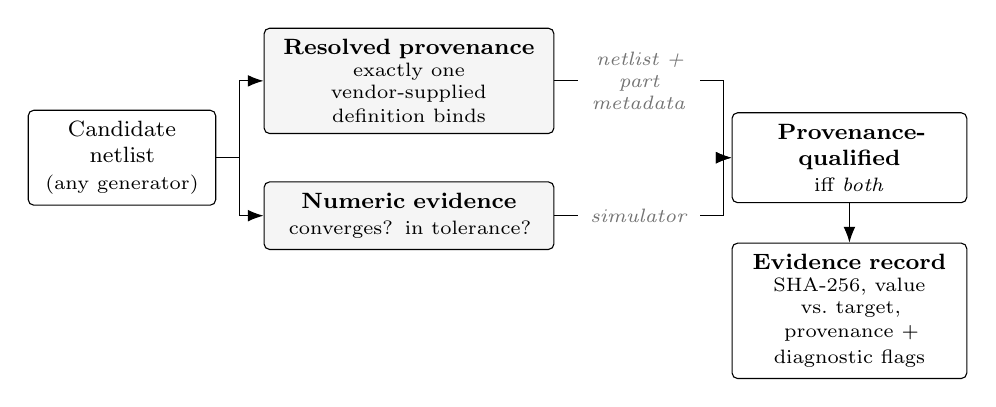
\begin{tikzpicture}[
  font=\footnotesize,
  box/.style={draw, rounded corners=2pt, align=center, inner sep=4pt,
              minimum height=7mm},
  lay/.style={box, fill=black!4, text width=34mm},
  dec/.style={box, text width=27mm},
  note/.style={font=\scriptsize\itshape, text=black!55, align=center},
  ar/.style={-{Latex[length=2mm]}, thin}
]

% Candidate Netlist Node
\node[box, text width=21mm] (net) {Candidate\\netlist\\\scriptsize(any generator)};

% Qualification predicates
\node[lay, above right=3mm and 6mm of net.east, anchor=south west] (l1)
  {\textbf{Resolved provenance}\\
   \scriptsize exactly one vendor-supplied\\[-1pt]
   \scriptsize definition binds};
\node[lay, below right=3mm and 6mm of net.east, anchor=north west] (l2)
  {\textbf{Numeric evidence}\\
   \scriptsize converges? in tolerance?};

% Note Nodes
\node[note, right=3mm of l1.east, text width=13mm] (n1) {netlist +\\part metadata};
\node[note, right=3mm of l2.east, text width=13mm] (n2) {simulator};

% Qualification Node
\node[dec, right=4mm of n1.east |- net.center] (acc)
  {\textbf{Provenance-qualified}\\\scriptsize iff \emph{both}};

% Evidence Record Node
\node[box, below=5mm of acc, text width=27mm] (rec)
  {\textbf{Evidence record}\\
   \scriptsize SHA-256, value vs.\ target,\\[-1pt]
   \scriptsize provenance + diagnostic flags};

% Routing Arrows

% 1. From the netlist to the two qualification predicates
\draw[ar] (net.east) -- ++(3mm,0) |- (l1.west);
\draw[ar] (net.east) -- ++(3mm,0) |- (l2.west);

% 2. From the predicates to the inline text notes
\draw (l1.east) -- (n1.west);
\draw (l2.east) -- (n2.west);

% 3. From the inline text notes to the qualification block
\draw[ar] (n1.east) -- ++(3mm,0) |- (acc.west);
\draw[ar] (n2.east) -- ++(3mm,0) |- (acc.west);

% 4. From the qualification block to the evidence record
\draw[ar] (acc.south) -- (rec.north);

\end{tikzpicture}
\caption{The provenance-aware evaluation framework. A numeric pass is
  provenance-qualified only when the requested part name also resolves to
  exactly one vendor-supplied definition. The evidence record additionally
  carries pin-role and waveform-integrity diagnostics, but those signals do
  not feed the qualification decision because they add no correct rejection
  on this corpus. Provenance qualification is stronger than numeric acceptance
  and deliberately narrower than general circuit verification.}
\label{fig:protocol}
\end{figure}

\paragraph{Resolved model provenance.}
The audit uses only the emitted netlist and trusted part metadata. It expands
\texttt{.lib}/\texttt{.include} directives transitively through the
simulator's search path, visits each resolved file once, and resolves the
requested name against the elaborated hierarchy. Qualification requires
exactly one reachable vendor definition; missing or mismatched files, local
shadowing, and duplicates therefore fail, while a wrapper that instantiates
the genuine part remains valid. Base-part matching catches renamed stubs; an
encrypted binding is hash-pinned and marked \texttt{opaque}.

\paragraph{Numeric evidence and diagnostics.}
The numeric conjunct requires convergence and every stated target, but remains
limited by specification richness and testbench ownership. Substitution,
stubbing, absence, pin-role, and waveform signals explain failures; none adds
a correct rejection beyond resolved binding here, and pin role has only
\MutPinPermuteRate{}\% held-out recall. They are reported as diagnostics, not
qualification gates.

\paragraph{Evidence and implementation.}
The record contains the candidate hash, directive resolutions and hashes, the
bound model and \texttt{opaque} status, measurements, simulator version, and
per-predicate verdicts. Library-relative paths protect user directories; hashes
make the decision re-derivable. Figure~\ref{fig:protocol} shows the whole gate; a full
trace is in Appendix~\ref{app:trace}.

\section{Artifact}
\label{sec:artifact}

The release contains the 20 cases, all \CorpusTotal{} raw generations and
netlists, audit records, grades, mutants, and analysis code. One command
re-audits the stored files, regenerates every table, and stops on seven corpus
integrity failures (Appendix~\ref{app:artifact}). LTspice and the vendor
library are required but freely available; model hashes expose installation
differences. Artifact: \artifacturl.

\section{Scope of the Qualification Claim}
\label{sec:scope}

Qualification establishes vendor-model provenance, not correct wiring,
transistor-level truth, manufacturability, or corner/noise/reliability
performance. Pin-role checking is partial (\MutPinPermuteRate{}\% held-out
recall), and \ProvFN{}/\StageProvAccepted{} qualified passes remain causally
false. The scope is single-part LTspice macro-model tasks, three LLMs,
$k=\SamplesPerCell{}$, and one scalar per case.

Absolute numeric rates also reflect candidate-authored testbenches; the prompt
ablation omits the joint factor cell, \NumNoCompletion{} attempts return no
completion, and \GroundsFakeRead{} false plus \GroundsValidRead{} valid grades
depend on one unblinded rater. Appendix~\ref{app:scope} gives the full limits
and sensitivity analysis.

\section{Conclusion}
\label{sec:conclusion}

A numeric gate certifies that a number was produced, not that the named part
produced it: \BareFalse{}/\BarePasses{} unprompted passes are false, and Pass@1
falls from \PassOneBareNumeric{}\% to \PassOneBareProv{}\% under provenance
qualification. An explicit no-substitution requirement increases library
references from \FactBareRefRate{}\% to \FactRequirementRefRate{}\%, but only
\FactRequirementResRate{}\% resolve, versus \FactLibraryResRate{}\% when the
directive is supplied. Resolved binding detects \ProvTP{}/\FalseAcceptTotal{}
false passes and every held-out provenance mutation; the interface diagnostic
catches \MutPinPermuteRate{}\% of pin permutations. Yet
\ProvFN{}/\StageProvAccepted{} qualified passes remain causally false.
Numerical Pass@$k$ should therefore be accompanied by provenance-qualified
Pass@$k$ and its residual false-acceptance rate, not read as general circuit
correctness.

\bibliographystyle{unsrtnat}
\bibliography{sample-base,provenance_refs}

\clearpage
\appendix
\section{Component-wise audit scores}
\label{app:ablation}

\begin{table}[t]
\centering
\caption{Every audit signal scored over the same \NumNumericPass{} numeric
  passes against the manual grades (\FalseAcceptTotal{} graded false
  acceptances, \LabelledReal{} graded valid). \emph{Ladder} rungs are unions
  of the predicates named, so a rung can only add detections to the one above
  it. \emph{Standalone} scores each predicate alone; \emph{Unique} is the
  detections lost when it is removed from the combined diagnostic union,
  i.e.\ what only it catches. \emph{Flagged} is always TP${}+{}$FP. Grades
  were assigned from the netlist without reference to the audit output. Only
  resolved binding defines provenance qualification; the remaining rows
  analyse diagnostic signals.}
\label{tab:ladder}
\small
\begin{tabular}{@{}lccccccc@{}}
\toprule
\textbf{Check} & \textbf{Flagged} & \textbf{TP} & \textbf{FP} &
  \textbf{Prec.} & \textbf{Rec.} & \textbf{Unique} \\
\midrule
\multicolumn{7}{@{}l}{\emph{Ladder} (cumulative)} \\
numeric simulation alone & 0 & 0 & 0 & N/A & 0\% & N/A \\
$+$ requested-part instance check & \SoloNoPartFlagged{} & \SoloNoPartTP{} & \SoloNoPartFP{}
  & \SoloNoPartPrecision{}\% & \SoloNoPartRecall{}\% & N/A \\
$+$ local same-name \texttt{.subckt} & 70 & 70 & 0 & 100\% & 89\% & N/A \\
$+$ behavioural-stub refinement & 70 & 70 & 0 & 100\% & 89\% & N/A \\
resolved-binding provenance (alone) & \SoloResolvedBindingFlagged{} & \ProvTP{} & \ProvFP{}
  & \ProvPrecision{}\% & \ProvRecall{}\% & N/A \\
$+$ pin-role diagnostic (combined union) & \AuditFlagged{} & \ConfTP{} & \ConfFP{}
  & \AuditPrecision{}\% & \AuditRecall{}\% & N/A \\
\midrule
\multicolumn{7}{@{}l}{\emph{Standalone} (each predicate alone)} \\
requested part never instantiated & \SoloNoPartFlagged{} & \SoloNoPartTP{}
  & \SoloNoPartFP{} & \SoloNoPartPrecision{}\% & \SoloNoPartRecall{}\%
  & \UniqueNoPart{} \\
local same-name \texttt{.subckt} & \SoloSubstitutedFlagged{} & \SoloSubstitutedTP{}
  & \SoloSubstitutedFP{} & \SoloSubstitutedPrecision{}\% & \SoloSubstitutedRecall{}\%
  & \UniqueSubstituted{} \\
local definition, no device content & \SoloBehavioralStubFlagged{}
  & \SoloBehavioralStubTP{} & \SoloBehavioralStubFP{}
  & \SoloBehavioralStubPrecision{}\% & \SoloBehavioralStubRecall{}\%
  & \UniqueBehavioralStub{} \\
name does not resolve to a vendor model & \SoloResolvedBindingFlagged{}
  & \SoloResolvedBindingTP{} & \SoloResolvedBindingFP{}
  & \SoloResolvedBindingPrecision{}\% & \SoloResolvedBindingRecall{}\%
  & \UniqueResolvedBinding{} \\
pin role disagrees with reference & \SoloPinRoleMismatchFlagged{}
  & \SoloPinRoleMismatchTP{} & \SoloPinRoleMismatchFP{}
  & \SoloPinRoleMismatchPrecision{}\% & \SoloPinRoleMismatchRecall{}\%
  & \UniquePinRoleMismatch{} \\
\bottomrule
\end{tabular}
\end{table}

Two consequences follow, in opposite directions. The useful part of this audit
is one carefully framed question: \emph{does the name bind to a
vendor-supplied definition?} This is why \S\ref{sec:protocol} states
the core qualification in those terms rather than as a list of detectors. But the naive
versions of that question are materially weaker: instance presence alone
reaches \SoloNoPartRecall{}\% recall, and the local-\texttt{.subckt} check a
reader might assume equivalent reaches \SoloSubstitutedRecall{}\%, because it
treats a written \texttt{.lib} directive as evidence the file exists. The
other predicates are retained because they decompose \emph{why} provenance
failed, and because they fire on the wider corpus (\FlagPinRole{} pin-role
flags over \NumNetlists{} netlists).

The smallest predicate subset matching the combined diagnostic union's recall has
\MinimalSubsetSize{} member (resolved-binding provenance) at
\MinimalSubsetFP{} false positives. Because the combined diagnostic flag is
the union of its predicates, and every other predicate's true detections are a
subset of that one's on this population, no predicate has a non-zero
\emph{Unique} true-positive count. Pin-role contributes only the single false
positive. The
standalone recalls show why the naive substitutes are weaker: a
local-\texttt{.subckt} check treats a written \texttt{.lib} directive as
evidence the file exists, and misses the netlists whose directive names a file
that is not there.

\section{Held-out mutation suite}
\label{app:mutants}

The predicates above were written while looking at this corpus, so their
performance on it measures fit. We therefore score them on an independent set
whose labels follow from construction rather than judgement: \MutParts{}
vendor parts appearing in no case here, each vendor reference netlist mutated
into \MutClasses{} variants (Appendix~\ref{app:mutants}). Seven mutations
destroy provenance or interface correctness, including the three cases a
static check is most likely to get wrong: a stub under a variant part name, a
genuine directive \emph{shadowed} by a local definition of the same name, and
a directive retargeted at a file that resolves but defines a different part.
Two preserve validity and are the ones that matter for precision:
\texttt{identity} leaves the reference untouched, and \texttt{wrapper}
instantiates the genuine part inside a locally defined pass-through, so it
reads as a local definition of the part while the vendor model is still in the
elaborated circuit.

Across \MutTotal{} mutants, resolved binding alone scores
\MutProvPrecision{}\% precision and \MutProvRecall{}\% recall when the
interface-only class is included in the denominator. It catches every
provenance-destroying mutation, including all three adversarial resolution
cases, and neither valid class is flagged. Adding pin-role as a diagnostic
raises the combined score to \MutPrecision{}\% precision and
\MutRecall{}\% recall (\MutTP{} true positives, \MutFP{} false positives,
\MutFN{} misses). The remaining misses are concentrated in
\texttt{pin\_permute}: transposing two nets on the instance is caught
\MutPinPermuteRate{}\% of the time because a transposition between two signal
pins is invisible to the permissive role comparison. Provenance and interface
therefore generalise differently: the provenance predicate transfers to
unseen parts essentially intact, while the interface check is a partial
diagnostic whose silence does not qualify a design.


\begin{table}[t]
\centering
\caption{Held-out validation. 40 vendor parts
  that appear in no probe case, each reference netlist mutated into
  9 variants whose label follows
  from the edit rather than from judgement. \emph{Flagged} is the combined
  provenance and interface diagnostic union. The two \emph{valid} rows are
  the test that matters for
  precision: \texttt{wrapper} instantiates the genuine part inside a locally
  defined pass-through, so it reads as a local definition while preserving
  provenance.}
\label{tab:mutants}
\small
\begin{tabular}{@{}llccc@{}}
\toprule
\textbf{Mutation} & \textbf{Label} & \textbf{$n$} & \textbf{Flagged} &
  \textbf{Rate} \\
\midrule
\texttt{identity} & valid & 40 & 0 & 0\% \\
\texttt{wrapper} & valid & 40 & 0 & 0\% \\
\texttt{substitute} & fake & 40 & 40 & 100\% \\
\texttt{renamed\_stub} & fake & 40 & 40 & 100\% \\
\texttt{shadow} & fake & 40 & 40 & 100\% \\
\texttt{drop\_library} & fake & 40 & 40 & 100\% \\
\texttt{remove\_part} & fake & 40 & 40 & 100\% \\
\texttt{alias\_file} & fake & 40 & 40 & 100\% \\
\texttt{pin\_permute} & fake & 40 & 22 & 55\% \\
\bottomrule
\end{tabular}
\end{table}

The parts come from the same vendor library as the main corpus, are parsed by
the same code, and the mutation operators were written by us after seeing that
corpus, so this is held-out validation over \emph{parts} within one
simulator/vendor ecosystem. It says nothing about transfer to another SPICE
dialect, another vendor's metadata conventions, or a naturally occurring
defect distribution.

Each mutation is a text edit over a vendor reference netlist, applied by
\texttt{bench/mutants.py}; the parts are drawn deterministically (fixed seed)
from the reference corpus after excluding every part used by a probe case, and
the full list of parts and per-mutant verdicts ships with the artifact.

\section{Framework trace}
\label{app:trace}

\begin{lstlisting}[language={}, caption={The provenance-aware framework driven end to end as
  tool calls on case D3. Elided fields are marked \texttt{...}; the full
  record is in the artifact. \texttt{submit} labels a result
  provenance-qualified only when the numeric targets are met \emph{and} the
  provenance binding resolves.},
  label={lst:trace}]
> find_template("AD8237")
  {"template": "data/templates/AD8237.net",
   "lib_directive": ".lib AD8237.lib"}

> simulate(netlist)
  {"converged": true, "log": "...", "raw": "D3.raw"}

> list_traces(netlist)
  {"traces": ["V(vout)", "V(vin+)", "V(vin-)", "V(vref)", ...]}

> verify_spec(netlist, [{"gain_db": 20.0, "tol": 1.0}])
  {"measured": {"gain_db": 20.0002}, "passed": true}

> audit_netlist(netlist, part="AD8237")
  {"binding": "vendor", "vendor_supplied": true, "opaque": false,
   "resolved_model_path": "<LTspice>/lib/sub/AD8237.lib",
   "resolved_model_sha256": "033cf879f17dd731...eb76c589",
   "local_definitions": [], "shadowed": false,
   "vendor_instance": "XU1 FB INN IN 0 VREF OUT VCC RG AD8237",
   "unresolved_directives": [], "flags": []}

> submit(netlist, part="AD8237")
  {"accepted": true,
   "evidence": {"netlist_sha256": "501b50ee2f33e40e...8fdf86c3",
                "simulator": "LTspice 17.2.4", ...}}
\end{lstlisting}
\section{Case suite and per-case results}
\label{app:cases}

Table~\ref{tab:cases} gives every case with its part, fake-risk stratum,
target and tolerance, and the per-arm outcome, so any individual result in the
released corpus can be located from the paper. Table~\ref{tab:nocomp} records
the generations lost to provider-side filtering per arm and model, which are
counted as failed attempts throughout (\S\ref{sec:results}).

\begin{table}[!ht]
\centering
\caption{The 20 cases. \emph{Risk} is how readily an ideal element reproduces
  the target number, the axis the suite is stratified on. For each arm:
  netlists returned over generations attempted, numeric passes, and passes
  graded as false acceptances (graded only for \textsc{bare} and
  \textsc{library}). C4 carries no numeric target and is excluded from every
  rate in the paper. Stimulus and load are chosen by the generating model
  (\S\ref{sec:design}); the specification text given to the model, and the
  reference netlist each case is graded against, ship with the artifact.}
\label{tab:cases}
\scriptsize
\setlength{\tabcolsep}{3.5pt}
\begin{tabular}{@{}llll ccc ccc ccc@{}}
\toprule
& & & & \multicolumn{3}{c}{\textsc{bare}} &
      \multicolumn{3}{c}{\textsc{library}} &
      \multicolumn{3}{c}{\textsc{requirement}} \\
\cmidrule(lr){5-7}\cmidrule(lr){8-10}\cmidrule(lr){11-13}
\textbf{Case} & \textbf{Part} & \textbf{Risk} & \textbf{Target} &
  Net & P & F & Net & P & F & Net & P & F \\
\midrule
A1 & \texttt{LT3045-1} & high & vout\_dc $= 3.3 \pm 0.1$ & 9/9 & 4 & 4 & 9/9 & 0 & N/A & 9/9 & 0 & N/A \\
A2 & \texttt{ADP7118} & high & vout\_dc $= 1.8 \pm 0.05$ & 9/9 & 5 & 5 & 9/9 & 0 & N/A & 9/9 & 0 & N/A \\
A3 & \texttt{LT3094} & high & vout\_dc $= -5 \pm 0.1$ & 9/9 & 5 & 5 & 9/9 & 0 & N/A & 9/9 & 0 & N/A \\
A4 & \texttt{ADR1399H} & high & vout\_dc $= 7.05 \pm 0.05$ & 6/9 & 3 & 3 & 6/9 & 5 & 0 & 9/9 & 0 & N/A \\
A5 & \texttt{LT6654-1.25} & high & vout\_dc $= 1.25 \pm 0.02$ & 9/9 & 6 & 6 & 6/9 & 0 & N/A & 9/9 & 0 & N/A \\
B1 & \texttt{AD8092} & medium & gain\_db $= 13.98 \pm 1$ & 9/9 & 4 & 4 & 9/9 & 3 & 2 & 9/9 & 0 & N/A \\
B2 & \texttt{ADA4177} & medium & gain\_db $= 20 \pm 1$ & 9/9 & 0 & N/A & 9/9 & 3 & 1 & 9/9 & 0 & N/A \\
B3 & \texttt{LTC6078} & medium & gain\_db $= 0 \pm 0.5$ & 9/9 & 1 & 1 & 9/9 & 3 & 0 & 9/9 & 0 & N/A \\
B4 & \texttt{AD8551} & medium & gain\_db $= 40 \pm 1$ & 9/9 & 5 & 3 & 9/9 & 5 & 1 & 9/9 & 0 & N/A \\
B5 & \texttt{MAX44245} & medium & gain\_db $= 26.02 \pm 1$ & 9/9 & 0 & N/A & 7/9 & 2 & 1 & 9/9 & 1 & N/A \\
C1 & \texttt{LTC6252} & high & gain\_db $= 6.02 \pm 1$ & 9/9 & 2 & 2 & 9/9 & 0 & N/A & 9/9 & 0 & N/A \\
C2 & \texttt{ADG5248F} & high & gain\_db $= 0 \pm 0.5$ & 9/9 & 6 & 6 & 9/9 & 0 & N/A & 9/9 & 0 & N/A \\
C3 & \texttt{LT8710} & high & vout\_dc $= 12 \pm 0.5$ & 9/9 & 3 & 3 & 9/9 & 0 & N/A & 6/9 & 0 & N/A \\
C4 & \texttt{AD4021} & high & inspection only & 9/9 & 0 & N/A & 6/9 & 0 & N/A & 4/9 & 0 & N/A \\
C5 & \texttt{LTC4281} & high & vout\_dc $= 12 \pm 0.5$ & 9/9 & 5 & 5 & 6/9 & 0 & N/A & 8/9 & 0 & N/A \\
D1 & \texttt{LT1720} & high & vout\_dc $= 0 \pm 0.3$ & 9/9 & 5 & 5 & 6/9 & 6 & 3 & 9/9 & 5 & N/A \\
D2 & \texttt{ADG711} & high & vout\_dc $= 2 \pm 0.1$ & 9/9 & 7 & 7 & 6/9 & 0 & N/A & 9/9 & 0 & N/A \\
D3 & \texttt{AD8237} & high & gain\_db $= 20 \pm 1$ & 9/9 & 2 & 2 & 9/9 & 0 & N/A & 9/9 & 0 & N/A \\
D4 & \texttt{LT6106} & high & vout\_dc $= 1 \pm 0.2$ & 9/9 & 6 & 6 & 9/9 & 0 & N/A & 8/9 & 0 & N/A \\
D5 & \texttt{ADR1399H} & high & vout\_dc $= 7.05 \pm 0.1$ & 9/9 & 4 & 4 & 3/9 & 0 & N/A & 9/9 & 0 & N/A \\
\bottomrule
\end{tabular}
\end{table}

\begin{table}[!ht]
\centering
\caption{Generations returning no completion under provider-side filtering,
  per arm and model. These are counted as failed attempts throughout
  (\S\ref{sec:results}), not as missing observations.}
\label{tab:nocomp}
\small
\begin{tabular}{@{}llcc@{}}
\toprule
\textbf{Arm} & \textbf{Model} & \textbf{Attempted} & \textbf{No completion} \\
\midrule
\textsc{bare} & \texttt{anthropic/claude-opus-5} & 60 & 3 \\
\textsc{bare} & \texttt{google/gemini-3.1-pro-preview} & 60 & 0 \\
\textsc{bare} & \texttt{openai/gpt-5.6-sol} & 60 & 0 \\
\textsc{library} & \texttt{anthropic/claude-opus-5} & 60 & 23 \\
\textsc{library} & \texttt{google/gemini-3.1-pro-preview} & 60 & 0 \\
\textsc{library} & \texttt{openai/gpt-5.6-sol} & 60 & 3 \\
\textsc{requirement} & \texttt{anthropic/claude-opus-5} & 60 & 0 \\
\textsc{requirement} & \texttt{google/gemini-3.1-pro-preview} & 60 & 6 \\
\textsc{requirement} & \texttt{openai/gpt-5.6-sol} & 60 & 4 \\
\bottomrule
\end{tabular}
\end{table}


\section{Per-model behaviour}
\label{app:permodel}

Table~\ref{tab:permodel} breaks the two graded arms down by model. It is the
evidence for the claim in \S\ref{sec:arms} that the gate is blind to a
specific generation strategy rather than uniformly unreliable: two models
stub heavily and false-accept at 100\% in \textsc{bare}, while the third
stubs once in 57 netlists.

\begin{table}[!ht]
\centering
\caption{Per model and arm. \emph{Att.} is generations attempted and
  \emph{Net.} netlists produced; the gap is provider-side filtering, which falls
  almost entirely on one model's \textsc{library} arm. Rates are over
  \emph{Net.} \emph{Stub} counts netlists defining a local subcircuit for the
  requested part with no device-level content.}
\label{tab:permodel}
\small
\setlength{\tabcolsep}{4pt}
\begin{tabular}{@{}llcccccc@{}}
\toprule
\textbf{Model} & \textbf{Arm} & \textbf{Att.} & \textbf{Net.} & \textbf{Pass} &
  \textbf{False} & \textbf{Genuine} & \textbf{Stub} \\
\midrule
\multirow{2}{*}{Claude Opus 5}
  & \textsc{bare}    & 57 & 54 & 37 & 100\% & 3  & 33 \\
  & \textsc{library} & 57 & 37 &  8 &   0\% & 37 &  0 \\
\multirow{2}{*}{GPT-5.6}
  & \textsc{bare}    & 57 & 57 & 32 & 100\% & 4  & 44 \\
  & \textsc{library} & 57 & 54 &  6 &   0\% & 52 &  0 \\
\multirow{2}{*}{Gemini 3.1 Pro}
  & \textsc{bare}    & 57 & 57 &  4 &  50\% & 12 &  1 \\
  & \textsc{library} & 57 & 57 & 13 &  62\% & 57 &  0 \\
\bottomrule
\end{tabular}
\end{table}

\section{Grounds recorded for each grade}
\label{app:grounds}

Table~\ref{tab:grounds} records what each of the \NumNumericPass{} grades
rests on, separating the \ConfTP{} grades a reader can re-derive mechanically
from the released file from the \GroundsFakeRead{} false and
\GroundsValidRead{} valid grades that required reading the netlist against the
criterion in \S\ref{sec:human}.

\begin{table}[!ht]
\centering
\caption{Grounds for each of the \NumNumericPass{} grades. \emph{Mechanical}
  grounds are re-derivable by any reader from the released netlist without
  judgement; the remainder were settled by reading the netlist against the
  criterion in \S\ref{sec:human}, and are the subset a single rater decided
  (\S\ref{sec:scope}).}
\label{tab:grounds}
\small
\begin{tabular}{@{}llc@{}}
\toprule
\textbf{Grade} & \textbf{Grounds} & \textbf{$n$} \\
\midrule
false acceptance & defines a local \texttt{.subckt} for the part, no vendor library loaded & \GroundsFakeSubckt{} \\
false acceptance & part never instantiated; named only in comments & \GroundsFakeNoInstance{} \\
false acceptance & settled by reading the netlist & \GroundsFakeRead{} \\
\midrule
valid    & vendor library loaded and part exercised; distortion measurement & \GroundsValidDistortion{} \\
valid    & settled by reading the netlist & \GroundsValidRead{} \\
\midrule
\multicolumn{2}{@{}l}{\emph{Total}} & \NumNumericPass{} \\
\bottomrule
\end{tabular}
\end{table}

\section{Prompts}
\label{app:prompts}

One system prompt is used in every arm and case: \emph{``You are an expert
analog applications engineer who writes LTspice netlists.''} The user prompt
differs across arms only in the block shown in bold below; everything else,
including the mandated node names and the instruction to include an analysis
directive, is identical. Case A1 is shown; other cases differ only in
\texttt{PART}, \texttt{REQUIREMENT}, and the target list, plus the supplied
directive in \textsc{library}.

\begin{lstlisting}[language={}, caption={The \textsc{bare} prompt (case A1).
  \textsc{requirement} and \textsc{library} insert one extra block at the
  marked point; nothing else changes.}, label={lst:prompt}]
Write a complete, simulation-ready LTspice netlist for the following
requirement.

PART: LT3045-1
REQUIREMENT: Low-dropout regulator stage delivering 3.3 V from a 5 V
input, supplying a 100 mA resistive load, with input and output
capacitors.

NUMERIC TARGETS:
  - vout_dc: target 3.3 (tolerance +/-0.1)

<<< arm-specific block inserted here; empty in BARE >>>

MANDATORY CONVENTIONS (the netlist will be run and measured
automatically):
  - Name the primary input node exactly: IN
  - Name the primary output node exactly: OUT
  - Include an analysis directive that lets the targets above be
    measured (a .tran run for DC/settled outputs, a .ac sweep or
    .tran with a SINE source for gain).
  - End the netlist with .end

Output the complete netlist and nothing else.
\end{lstlisting}

\begin{lstlisting}[language={}, caption={The two arm-specific blocks. Neither
  mentions the other's factor.}, label={lst:armblocks}]
=== REQUIREMENT (require, no availability) ===========================
PART FIDELITY REQUIREMENT:
  The netlist must instantiate the genuine LT3045-1 as a subcircuit.
  Do NOT define your own .subckt for the LT3045-1, and do not replace
  it with controlled sources or an idealised equivalent.

=== LIBRARY (availability, no requirement) ===========================
LIBRARY AVAILABILITY:
  The manufacturer's LTspice library is installed on this machine and
  on the simulator's search path, so the vendor macro-model for the
  LT3045-1 is available to instantiate as a subcircuit.
  Load it with:
    .lib LT3045-1.sub
\end{lstlisting}

\section{Extended scope discussion}
\label{app:scope}

This appendix gives the full reasoning behind the compressed points in
\S\ref{sec:scope}.

\paragraph{The candidate-authored testbench.}
Re-evaluating candidate subcircuits inside trusted, case-specific testbenches
is the natural strengthening of the behavioural layer, and it is not done
here. The provenance results do not depend on it: binding to a vendor
definition is decided from the file without simulation. However, the
numeric pass rates do, and should be read as properties of a permissive regime
rather than as circuit-quality estimates.

\paragraph{Provider-side filtering.}
The loss is condition- and model-dependent, rising with how explicitly the
prompt names a proprietary file, so it is not missing-at-random. Reporting
every rate over attempted generations removes the selection this would
otherwise introduce, at the cost of conflating a filtered request with a
failed one. We did not re-run through first-party APIs, so whether the
filtering belongs to the router or to the underlying models is not established
here.

\paragraph{Sensitivity to the judgement-dependent grades.}
Of the \NumNumericPass{} numeric passes, \ConfTP{} carry grades any reader can
re-derive from the released file. Re-grading all \GroundsFakeRead{}
judgement-dependent false grades as valid, the most adverse assumption
available, still leaves \ConfTP{}/\NumNumericPass{} false acceptances, so the
headline claim does not turn on them. The audit's \emph{recall} does: those
\ProvFN{} cases are exactly the ones the static check misses, so a regrade in
that direction would move recall while leaving precision untouched.
Independent expert regrading of that subset, and causal intervention (deleting
the named part and re-running the otherwise identical netlist) as a mechanical
substitute for judgement, are the two ways to settle it. Neither is done here,
and we do not claim the subset is settled.

\paragraph{What is checked.}
Every audit signal in \S\ref{sec:human} is a syntactic property of the
emitted netlist read against trusted part metadata: whether a subcircuit
bearing the part's name is defined locally, whether a library directive is
present, whether the part is instantiated, and whether each pin position
carries a net of the role the reference interface schema assigns. The first
three need the netlist alone; the pin-role check additionally needs that
schema, which is released with the artifact. None needs the generation trace
or an LLM judgement, so any reader can re-derive every signal from released
files without trusting our implementation. Signal integrity is checked separately from the simulated
waveform, via total harmonic distortion over the settled portion of the
transient record.

\paragraph{What the framework establishes, stated exactly.}
The qualification establishes model provenance: that the component the specification
named is the one instantiated, and that it is supplied by its manufacturer's
library rather than defined locally. The pin-role predicate is a non-gating
\emph{detector} of interface violations, not a proof of interface
correctness; it fires on a role disagreement but its silence carries no
guarantee (\S\ref{sec:heldout}). Neither qualification nor the diagnostics establish
transistor-level physical truth, and we do not claim they do. A
manufacturer-supplied macro-model may itself be substantially behavioural;
what distinguishes it from a locally written stub is authorship and
validation by the part's vendor, not the presence of device-level equations.

\paragraph{What lies outside any SPICE flow.}
Manufacturer-supplied macro-models for the parts in this suite ship as
encrypted binaries. Device-level operating points inside them, including the
saturation state of a particular transistor in an LT3045, are therefore not
observable to any tool operating on these models, ours included. A netlist
that instantiates the genuine part and meets its numeric target can be
provenance-qualified on that evidence; a correct interface and undistorted
output remain additional behavioural claims. Operating-region checks of
the kind used for open transistor-level designs require open device models
and are complementary to the provenance checks here.

\paragraph{Specification richness.}
Every case here is scored on a single scalar: 11 on a settled DC value, 8 on
a closed-loop gain. Whether a richer acceptance condition would close the gap
by itself is the natural next question, and this corpus cannot answer it. The
stored netlists carry the analysis directives their generators chose, so the
quantities needed for a second independent check are frequently not derivable
from them: no AC sweep with defined input and output nodes exists in the
gain-case runs, and total supply current in the DC-case runs is dominated by
load current rather than the part's own bias draw. Answering it requires
purpose-built testbenches per case rather than reanalysis of the existing
corpus, and we report the single-metric regime as the scope of the present
measurement rather than as a claim about simulator-based acceptance generally.

\section{Reproduction and compute}
\label{app:artifact}

Every figure in this paper is emitted by one command, which re-audits the
corpus from disk, recomputes each rate with its denominator, and writes the
macros the document uses:

\begin{lstlisting}[language=bash, caption={Regenerating every number in the
  paper.}, label={lst:repro}]
python bench/validate_cases.py            # corpus preflight
python bench/analyze.py   <RUN_ID>        # re-audit every stored netlist
python bench/reconcile.py <RUN_ID> \
       --out Neurips/generated            # tables + numbers.tex
\end{lstlisting}

\texttt{reconcile.py} refuses to emit if the corpus does not partition
(\CorpusTotal{} generations, \ArmAttempted{} per arm, \CorpusExcluded{}
inspection-only, \CorpusScored{} scored), if the status categories of the
\NumAttempted{} \textsc{bare}/\textsc{library} generations do not sum, if any denominator is zero, if a reported numeric pass has no
simulator artifact on disk, if grading labels conflict, or if a generation
identifier is duplicated.

\paragraph{Generation settings.}
Models are \texttt{anthropic/claude-opus-5}, \texttt{openai/gpt-5.6-sol} and
\texttt{google/gemini-3.1-pro-preview}, all reached through a single
commercial routing provider (OpenRouter) between 9 and 14 August 2026, with
one system prompt held constant across every arm and case. Sampling requests
temperature $0.7$ and a 32{,}000-token output budget; where a provider
rejects the temperature parameter the request is retried without it, and
where a reasoning model exhausts its budget before emitting visible text the
request is retried once at a larger budget. Generation is from scratch. No
reference netlist is shown, matching the setting the systems under discussion
operate in. The reference netlist is consulted only when grading and
when inferring pin roles. Simulation is LTspice 17.2.4 on macOS. Provider-side
filtering returns no completion for some requests; \S\ref{sec:results} treats
those as failed attempts rather than as missing observations, and
Appendix~\ref{app:cases} reports them per arm and model.

\paragraph{Compute resources.}
The reported experiment used no training or fine-tuning: it comprises
\CorpusTotal{} hosted inference requests at $k=3$, totalling approximately
25{,}400 seconds of endpoint wall time (47\,s per request on average). The
provider does not expose its worker hardware or memory. All local simulation
and analysis ran CPU-only on one macOS consumer laptop with LTspice 17.2.4;
no GPU is required, the stored corpus is under 1\,MB, and re-deriving every
table takes under two minutes without API access. Regenerating the corpus,
unlike reanalysis, requires access to the three hosted models.



\section{Extended prompt-ablation discussion}
\label{app:factorial}

\paragraph{Why Gemini does not respond to \textsc{requirement}.}
Of Gemini~3.1~Pro's \textsc{bare} netlists, only one in 57 defines a local
subcircuit for the requested part (\S\ref{sec:arms}); 46 instead instantiate
the part by name with no \texttt{.lib}/\texttt{.include} directive anywhere in
the file, an incomplete reference rather than a fabricated one. This is the detector's
\texttt{unresolvable\_part} diagnostic, not a suspect flag, since a netlist in
this state cannot converge and so cannot produce a false pass. A prohibition
against fabricating a local subcircuit cannot change the behaviour of a
model that was not fabricating one; Gemini's low \textsc{bare}
false-acceptance rate and its flat response to \textsc{requirement} reflect
the same underlying behaviour.

\paragraph{Content-filter escalation, full figures.}
For Claude Opus~5, out of 57 attempted generations per arm: \textsc{bare} loses
\FactBareClaudeNoComp{}; \textsc{requirement}, which forbids fabrication but
names no file, loses \FactRequirementClaudeNoComp{}; \textsc{library}, which
asserts the file exists and gives its path, loses \FactLibraryClaudeNoComp{}.
The no-completion rate is substantially higher in the condition that
explicitly names the proprietary file. We report the association only.

\newpage
\section*{NeurIPS Paper Checklist}

\begin{enumerate}

\item {\bf Claims}
    \item[] Question: Do the main claims made in the abstract and introduction accurately reflect the paper's contributions and scope?
    \item[] Answer: \answerYes{}
    \item[] Justification: The abstract and introduction report the same scoped quantities as the results: \BareFalse{}/\BarePasses{} false unprompted numeric passes, \FalseAcceptTotal{}/\NumNumericPass{} false numeric passes across the two manually graded arms, \ProvTP{}/\FalseAcceptTotal{} false passes detected by resolved binding at \ProvPrecision{}\% precision and \ProvRecall{}\% recall, and \ProvFN{}/\StageProvAccepted{} residual false provenance-qualified passes. Denominators and 95\% case-clustered bootstrap intervals are given in Tables~\ref{tab:main} and~\ref{tab:passk}; the three-model, 20-case, single-simulator/vendor scope is stated in Sections~\ref{sec:design} and~\ref{sec:scope}.
    \item[] Guidelines:
    \begin{itemize}
        \item The answer \answerNA{} means that the abstract and introduction do not include the claims made in the paper.
        \item The abstract and/or introduction should clearly state the claims made, including the contributions made in the paper and important assumptions and limitations. A \answerNo{} or \answerNA{} answer to this question will not be perceived well by the reviewers. 
        \item The claims made should match theoretical and experimental results, and reflect how much the results can be expected to generalize to other settings. 
        \item It is fine to include aspirational goals as motivation as long as it is clear that these goals are not attained by the paper. 
    \end{itemize}

\item {\bf Limitations}
    \item[] Question: Does the paper discuss the limitations of the work performed by the authors?
    \item[] Answer: \answerYes{}
    \item[] Justification: Section~\ref{sec:scope} is a dedicated limitations section. It distinguishes provenance qualification from correct wiring, transistor-level truth, manufacturability, and corner/noise/reliability verification; notes the partial held-out recall of the pin-role diagnostic and the \ProvFN{}/\StageProvAccepted{} residual false qualified passes; and bounds the study to three models, 20 single-part cases, one scalar per case, $k=3$, one simulator, and one vendor ecosystem. It also discloses candidate-authored testbenches, the incomplete three-arm rather than full $2\times2$ prompt ablation, no-completion outcomes, and one unblinded manual grader; Appendix~\ref{app:scope} expands these limitations and the adverse regrading sensitivity analysis.
    \item[] Guidelines:
    \begin{itemize}
        \item The answer \answerNA{} means that the paper has no limitation while the answer \answerNo{} means that the paper has limitations, but those are not discussed in the paper. 
        \item The authors are encouraged to create a separate ``Limitations'' section in their paper.
        \item The paper should point out any strong assumptions and how robust the results are to violations of these assumptions (e.g., independence assumptions, noiseless settings, model well-specification, asymptotic approximations only holding locally). The authors should reflect on how these assumptions might be violated in practice and what the implications would be.
        \item The authors should reflect on the scope of the claims made, e.g., if the approach was only tested on a few datasets or with a few runs. In general, empirical results often depend on implicit assumptions, which should be articulated.
        \item The authors should reflect on the factors that influence the performance of the approach. For example, a facial recognition algorithm may perform poorly when image resolution is low or images are taken in low lighting. Or a speech-to-text system might not be used reliably to provide closed captions for online lectures because it fails to handle technical jargon.
        \item The authors should discuss the computational efficiency of the proposed algorithms and how they scale with dataset size.
        \item If applicable, the authors should discuss possible limitations of their approach to address problems of privacy and fairness.
        \item While the authors might fear that complete honesty about limitations might be used by reviewers as grounds for rejection, a worse outcome might be that reviewers discover limitations that aren't acknowledged in the paper. The authors should use their best judgment and recognize that individual actions in favor of transparency play an important role in developing norms that preserve the integrity of the community. Reviewers will be specifically instructed to not penalize honesty concerning limitations.
    \end{itemize}

\item {\bf Theory assumptions and proofs}
    \item[] Question: For each theoretical result, does the paper provide the full set of assumptions and a complete (and correct) proof?
    \item[] Answer: \answerNA{}
    \item[] Justification: The paper contains no theoretical results. Equations~\ref{eq:gate} and~\ref{eq:provqual} define the measured numeric and provenance-qualified acceptance criteria; no theorem, lemma, or proof is claimed.
    \item[] Guidelines:
    \begin{itemize}
        \item The answer \answerNA{} means that the paper does not include theoretical results. 
        \item All the theorems, formulas, and proofs in the paper should be numbered and cross-referenced.
        \item All assumptions should be clearly stated or referenced in the statement of any theorems.
        \item The proofs can either appear in the main paper or the supplemental material, but if they appear in the supplemental material, the authors are encouraged to provide a short proof sketch to provide intuition. 
        \item Inversely, any informal proof provided in the core of the paper should be complemented by formal proofs provided in appendix or supplemental material.
        \item Theorems and Lemmas that the proof relies upon should be properly referenced. 
    \end{itemize}

    \item {\bf Experimental result reproducibility}
    \item[] Question: Does the paper fully disclose all the information needed to reproduce the main experimental results of the paper to the extent that it affects the main claims and/or conclusions of the paper (regardless of whether the code and data are provided or not)?
    \item[] Answer: \answerYes{}
    \item[] Justification: Section~\ref{sec:design} specifies the 20-case suite, the exact \textsc{bare}/\textsc{requirement}/\textsc{library} prompt differences, three models, $k=3$, and the scoring and grading protocol. The corpus identity is stated once: \CorpusTotal{} attempted generations, \CorpusExcluded{} inspection-only generations, and \CorpusScored{} scored generations. Appendix~\ref{app:artifact} gives exact model identifiers, dates, temperature, output budget, retry policy, LTspice version, integrity checks, and commands that re-audit stored netlists and regenerate every table. The intended artifact includes raw responses, netlists, simulator outputs, audit records, grades, mutants, and analysis code, so verification does not require repeating hosted inference.
    \item[] Guidelines:
    \begin{itemize}
        \item The answer \answerNA{} means that the paper does not include experiments.
        \item If the paper includes experiments, a \answerNo{} answer to this question will not be perceived well by the reviewers: Making the paper reproducible is important, regardless of whether the code and data are provided or not.
        \item If the contribution is a dataset and\slash or model, the authors should describe the steps taken to make their results reproducible or verifiable. 
        \item Depending on the contribution, reproducibility can be accomplished in various ways. For example, if the contribution is a novel architecture, describing the architecture fully might suffice, or if the contribution is a specific model and empirical evaluation, it may be necessary to either make it possible for others to replicate the model with the same dataset, or provide access to the model. In general. releasing code and data is often one good way to accomplish this, but reproducibility can also be provided via detailed instructions for how to replicate the results, access to a hosted model (e.g., in the case of a large language model), releasing of a model checkpoint, or other means that are appropriate to the research performed.
        \item While NeurIPS does not require releasing code, the conference does require all submissions to provide some reasonable avenue for reproducibility, which may depend on the nature of the contribution. For example
        \begin{enumerate}
            \item If the contribution is primarily a new algorithm, the paper should make it clear how to reproduce that algorithm.
            \item If the contribution is primarily a new model architecture, the paper should describe the architecture clearly and fully.
            \item If the contribution is a new model (e.g., a large language model), then there should either be a way to access this model for reproducing the results or a way to reproduce the model (e.g., with an open-source dataset or instructions for how to construct the dataset).
            \item We recognize that reproducibility may be tricky in some cases, in which case authors are welcome to describe the particular way they provide for reproducibility. In the case of closed-source models, it may be that access to the model is limited in some way (e.g., to registered users), but it should be possible for other researchers to have some path to reproducing or verifying the results.
        \end{enumerate}
    \end{itemize}


\item {\bf Open access to data and code}
    \item[] Question: Does the paper provide open access to the data and code, with sufficient instructions to faithfully reproduce the main experimental results, as described in supplemental material?
       \item[] Answer: \answerYes{}
    \item[] Justification: The release contains the case suite, all
    \CorpusTotal{} generations with raw responses and simulated netlists,
    per-netlist audit and measurement records with resolved include paths and
    model hashes, grading verdicts, the held-out mutation suite, and the
    analysis code, at \artifacturl{} (\S\ref{sec:artifact}). Resolved library
    paths in released evidence records are normalised to a library-relative
    form so that no operating user's home directory is disclosed. Reproduction
    requires LTspice and the vendor library, both free downloads from the
    manufacturer; the vendor macro-models are not redistributed, so the corpus
    is reconstructed from the reader's own installation
    \item[] Guidelines:
    \begin{itemize}
        \item The answer \answerNA{} means that paper does not include experiments requiring code.
        \item Please see the NeurIPS code and data submission guidelines (\url{https://neurips.cc/public/guides/CodeSubmissionPolicy}) for more details.
        \item While we encourage the release of code and data, we understand that this might not be possible, so \answerNo{} is an acceptable answer. Papers cannot be rejected simply for not including code, unless this is central to the contribution (e.g., for a new open-source benchmark).
        \item The instructions should contain the exact command and environment needed to run to reproduce the results. See the NeurIPS code and data submission guidelines (\url{https://neurips.cc/public/guides/CodeSubmissionPolicy}) for more details.
        \item The authors should provide instructions on data access and preparation, including how to access the raw data, preprocessed data, intermediate data, and generated data, etc.
        \item The authors should provide scripts to reproduce all experimental results for the new proposed method and baselines. If only a subset of experiments are reproducible, they should state which ones are omitted from the script and why.
        \item At submission time, to preserve anonymity, the authors should release anonymized versions (if applicable).
        \item Providing as much information as possible in supplemental material (appended to the paper) is recommended, but including URLs to data and code is permitted.
    \end{itemize}


\item {\bf Experimental setting/details}
    \item[] Question: Does the paper specify all the training and test details (e.g., data splits, hyperparameters, how they were chosen, type of optimizer) necessary to understand the results?
    \item[] Answer: \answerYes{}
    \item[] Justification: No training or optimization is performed. Section~\ref{sec:design} gives the three-arm ablation, corpus arithmetic, case construction, measurement rules, and $k=3$ independent attempts per case/model/arm. Appendix~\ref{app:artifact} identifies the three hosted model endpoints and routing provider, dates the requests, and reports temperature $0.7$, a 32{,}000-token output budget, retry behavior, generation from scratch, and LTspice 17.2.4. Prompts are reproduced in Appendix~\ref{app:prompts}, and no-completion outcomes are retained as intention-to-treat failures rather than removed.
    \item[] Guidelines:
    \begin{itemize}
        \item The answer \answerNA{} means that the paper does not include experiments.
        \item The experimental setting should be presented in the core of the paper to a level of detail that is necessary to appreciate the results and make sense of them.
        \item The full details can be provided either with the code, in appendix, or as supplemental material.
    \end{itemize}

\item {\bf Experiment statistical significance}
    \item[] Question: Does the paper report error bars suitably and correctly defined or other appropriate information about the statistical significance of the experiments?
    \item[] Answer: \answerYes{}
    \item[] Justification: Table~\ref{tab:main} reports 95\% nonparametric bootstrap confidence intervals from 10{,}000 replicates that resample whole cases, preserving generations nested within a case. Table~\ref{tab:passk} reports paired case-clustered bootstrap intervals for the numeric-minus-provenance change, applying both criteria to the same resampled cases. The paper identifies cases as the sampling unit, states that models are pooled, gives every count and denominator, and makes no normality assumption.
    \item[] Guidelines:
    \begin{itemize}
        \item The answer \answerNA{} means that the paper does not include experiments.
        \item The authors should answer \answerYes{} if the results are accompanied by error bars, confidence intervals, or statistical significance tests, at least for the experiments that support the main claims of the paper.
        \item The factors of variability that the error bars are capturing should be clearly stated (for example, train/test split, initialization, random drawing of some parameter, or overall run with given experimental conditions).
        \item The method for calculating the error bars should be explained (closed form formula, call to a library function, bootstrap, etc.)
        \item The assumptions made should be given (e.g., Normally distributed errors).
        \item It should be clear whether the error bar is the standard deviation or the standard error of the mean.
        \item It is OK to report 1-sigma error bars, but one should state it. The authors should preferably report a 2-sigma error bar than state that they have a 96\% CI, if the hypothesis of Normality of errors is not verified.
        \item For asymmetric distributions, the authors should be careful not to show in tables or figures symmetric error bars that would yield results that are out of range (e.g., negative error rates).
        \item If error bars are reported in tables or plots, the authors should explain in the text how they were calculated and reference the corresponding figures or tables in the text.
    \end{itemize}

\item {\bf Experiments compute resources}
    \item[] Question: For each experiment, does the paper provide sufficient information on the computer resources (type of compute workers, memory, time of execution) needed to reproduce the experiments?
    \item[] Answer: \answerYes{}
    \item[] Justification: Appendix~\ref{app:artifact} reports \CorpusTotal{} hosted inference requests, approximately 25{,}400 seconds of endpoint wall time (47 seconds per request on average), and explicitly states that the routing provider does not expose worker hardware or memory. Local simulation and analysis used LTspice 17.2.4 CPU-only on one macOS consumer laptop with no GPU; the corpus is under 1\,MB and complete reanalysis takes under two minutes without API access. No training or fine-tuning was performed. These disclosures distinguish the cost of regenerating the hosted corpus from the much smaller cost of reproducing the reported tables from released artifacts.
    \item[] Guidelines:
    \begin{itemize}
        \item The answer \answerNA{} means that the paper does not include experiments.
        \item The paper should indicate the type of compute workers CPU or GPU, internal cluster, or cloud provider, including relevant memory and storage.
        \item The paper should provide the amount of compute required for each of the individual experimental runs as well as estimate the total compute. 
        \item The paper should disclose whether the full research project required more compute than the experiments reported in the paper (e.g., preliminary or failed experiments that didn't make it into the paper). 
    \end{itemize}
    
\item {\bf Code of ethics}
    \item[] Question: Does the research conducted in the paper conform, in every respect, with the NeurIPS Code of Ethics \url{https://neurips.cc/public/EthicsGuidelines}?
        \item[] Answer: \answerYes{}
    \item[] Justification: The research conforms to the NeurIPS Code of
    Ethics. It evaluates hosted language models on an engineering task using
    publicly available vendor macro-models, involves no human subjects and no
    personal data, and redistributes no proprietary vendor models.
    \item[] Guidelines:
    \begin{itemize}
        \item The answer \answerNA{} means that the authors have not reviewed the NeurIPS Code of Ethics.
        \item If the authors answer \answerNo, they should explain the special circumstances that require a deviation from the Code of Ethics.
        \item The authors should make sure to preserve anonymity (e.g., if there is a special consideration due to laws or regulations in their jurisdiction).
    \end{itemize}


\item {\bf Broader impacts}
    \item[] Question: Does the paper discuss both potential positive societal impacts and negative societal impacts of the work performed?
    \item[] Answer: \answerYes{}
    \item[] Justification: Sections~\ref{sec:intro}, \ref{sec:scope}, and~\ref{sec:conclusion} describe the principal positive impact: provenance-qualified reporting can reduce misleading simulator-only success claims in AI-assisted hardware workflows. They also state the main misuse risk: users may over-read a provenance-qualified numeric pass as proof of correct wiring, transistor-level behavior, manufacturability, or reliability even though \ProvFN{}/\StageProvAccepted{} qualified passes remain false under manual grading. The proposed mitigation is to report provenance qualification and residual false acceptance alongside numeric Pass@$k$, while keeping interface and waveform checks explicitly labeled as diagnostics.
    \item[] Guidelines:
    \begin{itemize}
        \item The answer \answerNA{} means that there is no societal impact of the work performed.
        \item If the authors answer \answerNA{} or \answerNo, they should explain why their work has no societal impact or why the paper does not address societal impact.
        \item Examples of negative societal impacts include potential malicious or unintended uses (e.g., disinformation, generating fake profiles, surveillance), fairness considerations (e.g., deployment of technologies that could make decisions that unfairly impact specific groups), privacy considerations, and security considerations.
        \item The conference expects that many papers will be foundational research and not tied to particular applications, let alone deployments. However, if there is a direct path to any negative applications, the authors should point it out. For example, it is legitimate to point out that an improvement in the quality of generative models could be used to generate Deepfakes for disinformation. On the other hand, it is not needed to point out that a generic algorithm for optimizing neural networks could enable people to train models that generate Deepfakes faster.
        \item The authors should consider possible harms that could arise when the technology is being used as intended and functioning correctly, harms that could arise when the technology is being used as intended but gives incorrect results, and harms following from (intentional or unintentional) misuse of the technology.
        \item If there are negative societal impacts, the authors could also discuss possible mitigation strategies (e.g., gated release of models, providing defenses in addition to attacks, mechanisms for monitoring misuse, mechanisms to monitor how a system learns from feedback over time, improving the efficiency and accessibility of ML).
    \end{itemize}
    
\item {\bf Safeguards}
    \item[] Question: Does the paper describe safeguards that have been put in place for responsible release of data or models that have a high risk for misuse (e.g., pre-trained language models, image generators, or scraped datasets)?
    \item[] Answer: \answerNA{}
    \item[] Justification: The release contains no pretrained models, generative model weights, or scraped data. It consists of circuit specifications, model-generated SPICE netlists for single vendor parts, measurement and audit records, and analysis code, none of which carries a dual-use or misuse risk requiring gated release.
    \item[] Guidelines:
    \begin{itemize}
        \item The answer \answerNA{} means that the paper poses no such risks.
        \item Released models that have a high risk for misuse or dual-use should be released with necessary safeguards to allow for controlled use of the model, for example by requiring that users adhere to usage guidelines or restrictions to access the model or implementing safety filters. 
        \item Datasets that have been scraped from the Internet could pose safety risks. The authors should describe how they avoided releasing unsafe images.
        \item We recognize that providing effective safeguards is challenging, and many papers do not require this, but we encourage authors to take this into account and make a best faith effort.
    \end{itemize}

\item {\bf Licenses for existing assets}
    \item[] Question: Are the creators or original owners of assets (e.g., code, data, models), used in the paper, properly credited and are the license and terms of use explicitly mentioned and properly respected?
        \item[] Answer: \answerYes{}
    \item[] Justification: LTspice and the manufacturer-supplied macro-models
    are cited to their vendor (\cite{b16}) and are used under that vendor's
    free-distribution terms, which permit download and use but not
    redistribution. The artifact therefore records file identities and SHA-256
    hashes rather than shipping the models, and the reader supplies them from
    their own installation (\S\ref{sec:artifact}). Model access is through a
    commercial routing provider under its standard API terms, which permit
    research use of returned completions. All prior systems, datasets and
    benchmarks discussed are cited.
    \item[] Guidelines:
    \begin{itemize}
        \item The answer \answerNA{} means that the paper does not use existing assets.
        \item The authors should cite the original paper that produced the code package or dataset.
        \item The authors should state which version of the asset is used and, if possible, include a URL.
        \item The name of the license (e.g., CC-BY 4.0) should be included for each asset.
        \item For scraped data from a particular source (e.g., website), the copyright and terms of service of that source should be provided.
        \item If assets are released, the license, copyright information, and terms of use in the package should be provided. For popular datasets, \url{paperswithcode.com/datasets} has curated licenses for some datasets. Their licensing guide can help determine the license of a dataset.
        \item For existing datasets that are re-packaged, both the original license and the license of the derived asset (if it has changed) should be provided.
        \item If this information is not available online, the authors are encouraged to reach out to the asset's creators.
    \end{itemize}

\item {\bf New assets}
    \item[] Question: Are new assets introduced in the paper well documented and is the documentation provided alongside the assets?
        \item[] Answer: \answerYes{}
    \item[] Justification: The released assets are the 20-case suite, the
    generation corpus with raw responses and simulated netlists, the held-out
    mutation suite, the audit and reconciliation code, and the tool server,
    released under the MIT License. Their structure, regeneration commands and
    integrity guarantees are documented in \S\ref{sec:artifact} and
    Appendix~\ref{app:artifact}; the vendor macro-models are not
    redistributed, so no third-party license is re-issued.
    \item[] Guidelines:
    \begin{itemize}
        \item The answer \answerNA{} means that the paper does not release new assets.
        \item Researchers should communicate the details of the dataset\slash code\slash model as part of their submissions via structured templates. This includes details about training, license, limitations, etc. 
        \item The paper should discuss whether and how consent was obtained from people whose asset is used.
        \item At submission time, remember to anonymize your assets (if applicable). You can either create an anonymized URL or include an anonymized zip file.
    \end{itemize}

\item {\bf Crowdsourcing and research with human subjects}
    \item[] Question: For crowdsourcing experiments and research with human subjects, does the paper include the full text of instructions given to participants and screenshots, if applicable, as well as details about compensation (if any)? 
    \item[] Answer: \answerNA{}
    \item[] Justification: The paper involves no crowdsourcing and no human subjects. The manual grading in Section~\ref{sec:human} was performed by an author on model-generated netlists against the stated causal criterion, and Section~\ref{sec:scope} discloses that the rater was unblinded.
    \item[] Guidelines:
    \begin{itemize}
        \item The answer \answerNA{} means that the paper does not involve crowdsourcing nor research with human subjects.
        \item Including this information in the supplemental material is fine, but if the main contribution of the paper involves human subjects, then as much detail as possible should be included in the main paper. 
        \item According to the NeurIPS Code of Ethics, workers involved in data collection, curation, or other labor should be paid at least the minimum wage in the country of the data collector. 
    \end{itemize}

\item {\bf Institutional review board (IRB) approvals or equivalent for research with human subjects}
    \item[] Question: Does the paper describe potential risks incurred by study participants, whether such risks were disclosed to the subjects, and whether Institutional Review Board (IRB) approvals (or an equivalent approval/review based on the requirements of your country or institution) were obtained?
    \item[] Answer: \answerNA{}
    \item[] Justification: The study has no participants: it evaluates language-model outputs against a simulator, and the only human involvement is an author's grading of those outputs. No IRB review is applicable.
    \item[] Guidelines:
    \begin{itemize}
        \item The answer \answerNA{} means that the paper does not involve crowdsourcing nor research with human subjects.
        \item Depending on the country in which research is conducted, IRB approval (or equivalent) may be required for any human subjects research. If you obtained IRB approval, you should clearly state this in the paper. 
        \item We recognize that the procedures for this may vary significantly between institutions and locations, and we expect authors to adhere to the NeurIPS Code of Ethics and the guidelines for their institution. 
        \item For initial submissions, do not include any information that would break anonymity (if applicable), such as the institution conducting the review.
    \end{itemize}

\item {\bf Declaration of LLM usage}
    \item[] Question: Does the paper describe the usage of LLMs if it is an important, original, or non-standard component of the core methods in this research? Note that if the LLM is used only for writing, editing, or formatting purposes and does \emph{not} impact the core methodology, scientific rigor, or originality of the research, declaration is not required.
    \item[] Answer: \answerYes{}
    \item[] Justification: LLMs are the object of study. Section~\ref{sec:design} and Appendix~\ref{app:artifact} name Claude Opus 5, GPT-5.6, and Gemini 3.1 Pro, the routing provider, dates, sampling settings, and the \textsc{bare}/\textsc{requirement}/\textsc{library} conditions. The design contains \NumCases{} cases $\times$ \NumModels{} models $\times$ $k=\SamplesPerCell{}$ attempts $\times$ \CorpusArms{} arms $=\CorpusTotal{}$ generations. No-completion outcomes are retained as failures. No LLM performs provenance resolution, diagnostics, simulation measurement, grading aggregation, or statistical analysis; those components are deterministic or manually adjudicated as described in Sections~\ref{sec:human} and~\ref{sec:protocol}.
    \item[] Guidelines:
    \begin{itemize}
        \item The answer \answerNA{} means that the core method development in this research does not involve LLMs as any important, original, or non-standard components.
        \item Please refer to our LLM policy in the NeurIPS handbook for what should or should not be described.
    \end{itemize}

\end{enumerate}


\end{document}
